\documentclass[10pt]{article} 
%\IEEEoverridecommandlockouts                              
%\overrideIEEEmargins
\usepackage{url}
\usepackage{color,graphicx}
\usepackage{enumerate}
\usepackage{amssymb,amsmath,amsthm}
\usepackage[numbers]{natbib}
%\usepackage{algorithm2e}%
%\usepackage{almostfull}
\usepackage{booktabs}
%\usepackage[authoryear,round,longnamesfirst]{natbib}
%%% Environment for notation and a symbol command to go along with it.
%%% The argument should be the widest symbol which is expected if 
%%% \sym will be used to make the list.
%%%
\newenvironment{notation}[1]{%
\begin{list}{}{\small
\settowidth{\labelwidth}{{#1}\quad}%
\setlength{\itemsep}{1.5pt plus 0.5pt minus 0.2pt}%
\setlength{\parsep}{0ex}%
\setlength{\rightmargin}{0em}%
\setlength{\leftmargin}{\labelwidth}%
\addtolength{\leftmargin}{\labelsep}%
\addtolength{\leftmargin}{1em}}}{\end{list}}

\newcommand{\sym}[1]{\item[${#1}$\hfill{}]}

\newcommand{\bx}{\mathbf{x}}
\newcommand{\bu}{\mathbf{u}}
\newcommand{\bd}{\mathbf{d}}
\newcommand{\til}[1]{\tilde{#1}}
\newcommand{\norm}[1]{\vert #1 \vert}
\newcommand{\set}[1]{\left\lbrace #1 \right\rbrace}
\newcommand{\SetAlgoLined}{}

\newcommand{\I}{\mathcal{I}}
\newcommand{\BO}{\textrm{BO}}
\newcommand{\IP}{\textrm{Ip}}
\newcommand{\UP}{\textrm{Up}}
\newcommand{\DN}{\textrm{Dn}}
\newcommand{\Inv}{\textrm{Iv}}
\newcommand{\Dem}{\textrm{Dm}}
\newcommand{\ulambda}{\underline{\lambda}}
\newcommand{\olambda}{\overline{\lambda}}
\newcommand{\eig}{\text{eig}}
\newcommand{\diag}{\text{diag}}


\newtheorem{theorem}{Theorem}
\newtheorem{lemma}[theorem]{Lemma}
\newtheorem{proposition}[theorem]{Proposition}
\newtheorem{conjecture}[theorem]{Conjecture}
\newtheorem{corollary}[theorem]{Corollary}

\theoremstyle{definition}
\newtheorem{definition}[theorem]{Definition}
\newtheorem{remark}[theorem]{Remark}
\newtheorem{assumption}[theorem]{Assumption}
\newtheorem{hypothesis}[theorem]{Hypothesis}
\newtheorem{property}[theorem]{Property}



% add "Appendix" to the section heading
\newcommand{\appsection}[1]{\let\oldthesection\thesection
  \renewcommand{\thesection}{Appendix \oldthesection}
  \section{#1}\let\thesection\oldthesection}

\renewcommand\appendix{\par
\setcounter{section}{0}%
\setcounter{subsection}{0}%
\setcounter{table}{0}
\setcounter{figure}{0}
\gdef\thetable{\Alph{table}}
\gdef\thefigure{\Alph{figure}}
\gdef\thesection{\Alph{section}}
\setcounter{section}{0}}

\title{\LARGE \bf {Economic model predictive control for inventory management in
    supply chains}}
\author{Kaushik Subramanian\thanks{Department of Chemical and Biological Engineering, University
  of Wisconsin-Madison, U.S.A.} \and Christos T. Maravelias\footnotemark[1] \and James B. Rawlings
\thanks{Corresponding author: jbraw@engr.wisc.edu}\footnotemark[1]}


\begin{document}
\maketitle
\section{Introduction}
In this paper, we propose  economic model predictive
control (MPC) algorithm for inventory management in supply
chains with guaranteed closed-loop properties. We compare the
properties of the proposed controller with classical control policies
like the $(\sigma,\Sigma) $ policy. 

Over the past few years, there has been considerable interest in using
control theory to manage inventory in supply chains. See
\citet{sarimevis:patrinos:tarantilis:kiranoudis:2008,ortega:lin:2004}
for extensive reviews of control theory in supply chain
management. More recently, rolling horizon optimization and MPC-based
control approaches to supply chain optimization has been proposed \citep{
perealopez:ydstie:grossmann:2003,mestan:turkay:arkun:2006,dunbar:desa:2007a,
seferlis:giannelos:2004,kempf:2004,braun:rivera:carlyle:kempf:2002,Maestre:Pena:Camacho:2009}. While
closed-loop stability, or the stability of the dynamics of the supply
chain after implementing the proposed controller has been investigated
for inventory control using classical control theory, see for
instance
\citet{lin:wong:jang:shieh:chu:2004,venkateswaran:son:2005,hoberg:bradley:thonemann:2007};
the stability of supply chains using a model predictive controller has
not been studied extensively. Although stability theory for MPC is a
fairly mature field  \citep[Chapter 2]{rawlings:mayne:2009}, most
implementations of MPC for supply chains do not consider stability. In
\citet{subramanian:rawlings:maravelias:2012}, we proposed centralized
and cooperative MPC with stability and asymptotic convergence
guarantees for a  supply chain implementing MPC to track its
inventories to a set-point (safety stock). Our focus in this paper is to leverage
recent developments in Economic-MPC
\citep{amrit:rawlings:angeli:2011,diehl:amrit:rawlings:2011} to
develop a stable controller for inventory management in which the
controller directly optimizes the supply chain economics.

In Section \ref{sec:model}, we briefly describe the 2-node supply
chain that we shall use to illustrate the results in this paper. In
Section \ref{sec:economicMPC}, we review stability theory for economic
MPC and propose two flavors of MPC for
supply chain, (i) A pure economic objective function and (ii) A mixed
objective comprising of an economic objective and a tracking
objective. In Section \ref{sec:multi_example}, we implement the
controller proposed in this paper on a multi-product, multi-echelon
supply chain and compare the performance of the controller with that
of the $(\sigma,\Sigma) $ policy. In Section \ref{subsec:scheduling}, we
introduce a scheduling model for the manufacturing facility with the
aim of integrating scheduling and inventory control using MPC. We
present results on recursive feasibility using ideas from
\citet{subramanian:maravelias:rawlings:2012}. Finally, we present our
conclusions in Section \ref{sec:conclusions}.




\section{Two node supply chain}
\label{sec:model}
We study a two node supply chain comprising of a retailer and a
manufacturer (Figure \ref{fig:2stage}). The retailer responds to the customer demands which is
the external disturbance affecting the system. For the retailer,
labeled as node $1$, the state variables are $\Inv_1$ and $\BO_1$, the
inventory and backorder. Similarly, for the manufacturer, node $2$,
the state variables are $\Inv_2$ and $\BO_2$. The state of the supply
chain model therefore is $x = (\Inv_1,\BO_1,\Inv_2,\BO_2)'$. The inputs to the supply
chain model are the shipments and orders placed by each node,
$u = (S_{1c},O_{12},S_{21},O_{2p})'$, in which $S_{1C}$ is the
shipments delivered to the customer by node $1$, $O_{12}$ is the
orders placed by node $1$ to node $2$ while $S_{21}$ are the shipments
from the manufacturer to the retailer and $O_{2p}$ are the production
amounts of the manufacturer. The production delay is $2$ time units
while the shipment delay between the nodes is also $2$ units. We assume that
shipments are instantly delivered to the customers. The customer
demand is denoted by $d$ and the time instant by $k$. The inventory
and backorder material balance yields the dynamic equations for the
supply chain:
\begin{align*}
 \Inv_1(k+1) &= \Inv_1(k) + S_{21}(k-1) -S_{1c}(k) \\
 \BO_1(k+1) &= \BO_1(k) + d(k) -S_{1c}(k) \\
 \Inv_2(k+1) &= \Inv_2(k) + O_{2p}(k-2) -S_{21}(k) \\
 \BO_2(k+1) &= \BO_2(k) +O_{12}(k) - S_{21}(k)
\end{align*}

\begin{figure*}
\centering
\resizebox{0.9\textwidth}{!}{\begin{picture}(0,0)%
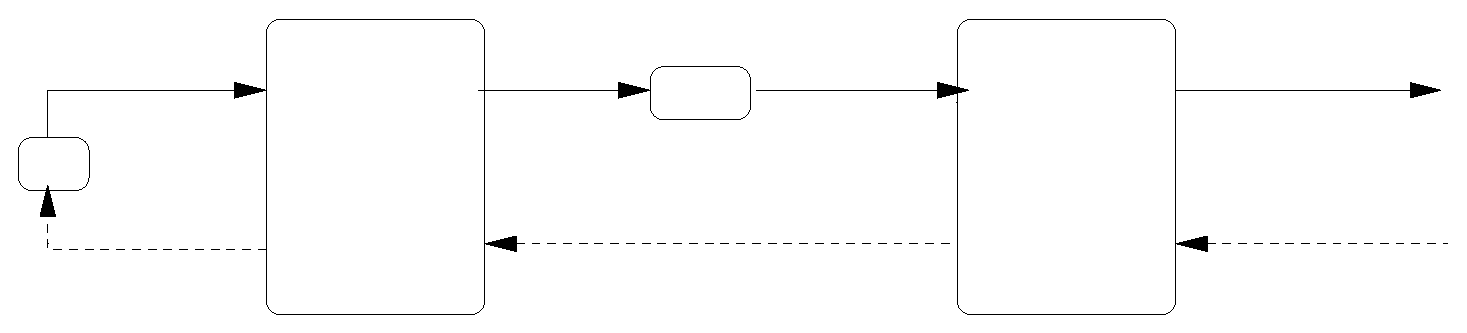
\includegraphics{2node}%
\end{picture}%
\setlength{\unitlength}{4144sp}%
%
\begingroup\makeatletter\ifx\SetFigFont\undefined%
\gdef\SetFigFont#1#2#3#4#5{%
  \reset@font\fontsize{#1}{#2pt}%
  \fontfamily{#3}\fontseries{#4}\fontshape{#5}%
  \selectfont}%
\fi\endgroup%
\begin{picture}(12701,2676)(166,-4459)
\put(9451,-2941){\makebox(0,0)[b]{\smash{{\SetFigFont{20}{24.0}{\familydefault}{\mddefault}{\updefault}{\color[rgb]{0,0,0}Retailer}%
}}}}
\put(181,-2266){\makebox(0,0)[lb]{\smash{{\SetFigFont{20}{24.0}{\familydefault}{\mddefault}{\updefault}{\color[rgb]{0,0,0}$S_{2p}(k-\tau_M)$}%
}}}}
\put(7066,-4291){\makebox(0,0)[lb]{\smash{{\SetFigFont{20}{24.0}{\familydefault}{\mddefault}{\updefault}{\color[rgb]{0,0,0}$O_{12}(k)$}%
}}}}
\put(811,-4291){\makebox(0,0)[lb]{\smash{{\SetFigFont{20}{24.0}{\familydefault}{\mddefault}{\updefault}{\color[rgb]{0,0,0}$S_{2p}(k)$}%
}}}}
\put(586,-3301){\makebox(0,0)[lb]{\smash{{\SetFigFont{20}{24.0}{\familydefault}{\mddefault}{\updefault}{\color[rgb]{0,0,0}$\tau_M = 2$}%
}}}}
\put(9451,-3571){\makebox(0,0)[b]{\smash{{\SetFigFont{20}{24.0}{\familydefault}{\mddefault}{\updefault}{\color[rgb]{0,0,0}Node $1$}%
}}}}
\put(3421,-3571){\makebox(0,0)[b]{\smash{{\SetFigFont{20}{24.0}{\familydefault}{\mddefault}{\updefault}{\color[rgb]{0,0,0}Node $2$}%
}}}}
\put(3421,-2941){\makebox(0,0)[b]{\smash{{\SetFigFont{20}{24.0}{\familydefault}{\mddefault}{\updefault}{\color[rgb]{0,0,0}Manufacturer}%
}}}}
\put(4591,-2311){\makebox(0,0)[lb]{\smash{{\SetFigFont{20}{24.0}{\familydefault}{\mddefault}{\updefault}{\color[rgb]{0,0,0}$S_{21}(k)$}%
}}}}
\put(5581,-2761){\makebox(0,0)[lb]{\smash{{\SetFigFont{20}{24.0}{\familydefault}{\mddefault}{\updefault}{\color[rgb]{0,0,0}$\tau_T=1$}%
}}}}
\put(10621,-2311){\makebox(0,0)[lb]{\smash{{\SetFigFont{20}{24.0}{\familydefault}{\mddefault}{\updefault}{\color[rgb]{0,0,0}$S_{1c}(k)$}%
}}}}
\put(11341,-4291){\makebox(0,0)[lb]{\smash{{\SetFigFont{20}{24.0}{\familydefault}{\mddefault}{\updefault}{\color[rgb]{0,0,0}$\Dem_{1c}(k)$}%
}}}}
\end{picture}%
}
\caption{Two-stage supply chain.}
\label{fig:2stage}
\end{figure*}

\paragraph{Remark.} Note that for centralized optimization of supply
chain operations, ordering between the nodes $O_{12}$ and the
backorder at the manufacturer $\BO_2$ are redundant. However, we use
this general model because it is the relevant model in distributed and
decentralized optimization frameworks.

\paragraph{Model.} We represent the supply chain model succinctly as
\begin{multline}
\label{eq:model0}
 x(k+1) = x(k)+\begin{bmatrix}B_{11}&B_{12}\\B_{21}&B_{22}\end{bmatrix}
 \begin{bmatrix}u_1(k)\\u_2(k)\end{bmatrix}+\\
 \begin{bmatrix}B_{11}^{(1)}&B_{12}^{(1)}\\B_{21}^{(1)}&B_{22}^{(1)}\end{bmatrix}
 \begin{bmatrix}u_1(k-1)\\u_2(k-1)\end{bmatrix}+
\\\begin{bmatrix}B_{11}^{(2)}&B_{12}^{(2)}\\B_{21}^{(2)}&B_{22}^{(2)}\end{bmatrix}
  \begin{bmatrix}u_1(k-2)\\u_2(k-2)\end{bmatrix}+B_dd(k)   
\end{multline}
in which $x = (\Inv_1,\BO_1,\Inv_2,\BO_2)'$ are the states, $u_1 = (S_{1c},O_{12})'$
and $u_2 = (S_{21},O_{1p})'$ are the inputs belonging to node $1$
(retailer) and node $2$ (supplier) respectively. The supply chain
model can be written as:
\begin{multline}
\label{eq:model}
\begin{bmatrix}x(k+1)\\u(k)\\u(k-1)\end{bmatrix} = 
\begin{bmatrix} I & B^{(1)} & B^{(2)} \\ 0&0 &0 \\0& I &0\end{bmatrix}
\begin{bmatrix}x(k)\\u(k-1)\\u(k-2)\end{bmatrix}\\
+\begin{bmatrix}B\\I\\0\end{bmatrix}u(k) + \begin{bmatrix}B_d\\0 \\0 \end{bmatrix}d(k)
\end{multline}

With a slight abuse of notation, we refer to the supply chain model as:
\[x(k+1) = Ax(k)+Bu(k)+B_dd(k)\]. The identity matrix is denoted as $I$.

\paragraph{Stage cost.} We define the economic stage cost as
\begin{equation}
\label{eq:ellE}
\ell_E(x,u) = q'x + r'u
\end{equation}
in which $q$ is a vector comprising of inventory holding $q_{\Inv_i}$
and lost sales $q_{\BO_i}$ costs, while $r$ is a vector comprising of
shipment costs (or negative profit) $r_{S_{1c}}, r_{S_{21}}$,
production costs $r_{O_{1p}}$ and ordering costs $r_{O_{12}}$. 

We also define a tracking stage cost as
\begin{equation}
\label{eq:ellT}
\ell_T(x,u,z_p) = (x-x_t)'Q(x-x_t)+(u-u_t)'R(u-u_t)
\end{equation}
in which $z_p = (x_t',u_t')'$ is a vector comprising of the state and
input targets $(x_t,u_t)$ respectively. The positive definite matrices
$Q,R$ penalize the deviation of the states and inputs from their
targets. In this paper, $Q,R>0$ are used as tuning parameters.

\paragraph{Constraints.} We assume that the input and states are
constrained to lie inside hyperboxes of the type $\underbar{x} \leq x
\leq \bar{x}$ and $\underbar{u} \leq u \leq \bar{u}$, in which the
inequalities are assigned componentwise. The constraints represent
storage capacity, non-negativity of states, shipping capacity etc.

\section{Economic MPC}
\label{sec:economicMPC}
\subsection{Rolling horizon optimization}
Given a planning horizon $N$ and demand forecast $\bd =
(d(k),d(k+1),\ldots,d(k+N-1))$, we formulate the following
optimization problem that is solved at time instance $k$
\begin{alignat}{1}
\label{eq:P}
\mathbb{P}(x(k)):& \min_{\bu}{V(\bu;x(k),\bd,N)} \nonumber \\
&\text{s.t~} x(i+1) = Ax(i) + Bu(i)+B_dd(i), \nonumber\\
&\underbar{x} \leq x(i) \leq \bar{x},  \\
&\underbar{u} \leq u(i) \leq \bar{u}, \nonumber \\
&i = k,k+1,\ldots,k+N-1\nonumber
\end{alignat}
in which $\bu = (u(k),u(k+1),\ldots,u(k+N-1))$. The cost function
$V(\bu;x(k),\bd,N)$ is the sum of $N$ stage costs
\[V(\bu;x(k),\bd,N) =  \sum_{i=0}^{k+N-1}
  \ell_E(x(k+i),u(k+i))\]
Upon obtaining the optimal solution $\bu^0(x(k);N,\bd)$, we inject the first input move
$u^0(k)$ and resolve the optimization problem
$\mathbb{P}(x(k+1))$. In figure \ref{fig:unstable_SC}, we show the
backorder evolution at the retailer for such a rolling horizon
implementation with  $N=15$, nominal demand $d(k)=10$ and the
following cost vector in which we assume that shipping costs are
greater than the backorder cost.
\[ q = (1,1,1,1)' \qquad r = (10,1,10,1)' \]
Clearly we can observe that despite implementing the optimal input at
each time instance, the backorder is increasing with time, indicating
that customer demand is not being met. Although, we have chosen a
pathological cost vector in which production costs are greater than
lost sales cost, we observe that there exists an unique steady-state
for this system $x_s = \underbar{x}=0, u_s = d$, that is the inventory
and backorders are zero and all the flows in the supply chain
(shipping and ordering between nodes, production) is equal to the
nominal demand.  The lower bounds on inventories and backorders are
zero. Notice that the choice of $u_s = d, x_s=0$ in \eqref{eq:model}
is a solution to:
\[ (I-I)x - B^{(1)}u-B^{(2)}u- Bu = B_dd \] 

Note that  the steady-state for the states in the supply
chain is independent of the demands and delays in the system.

For the costs mentioned
in above, staying at the steady-state incurs a cost of $220$ per period
which is much lesser than the cost incurred per period by the rolling
horizon controller is unbounded.

\begin{figure*}
\centering
\scriptsize
\resizebox{\textwidth}{!}{% GNUPLOT: LaTeX picture with Postscript
\begingroup
  \makeatletter
  \providecommand\color[2][]{%
    \GenericError{(gnuplot) \space\space\space\@spaces}{%
      Package color not loaded in conjunction with
      terminal option `colourtext'%
    }{See the gnuplot documentation for explanation.%
    }{Either use 'blacktext' in gnuplot or load the package
      color.sty in LaTeX.}%
    \renewcommand\color[2][]{}%
  }%
  \providecommand\includegraphics[2][]{%
    \GenericError{(gnuplot) \space\space\space\@spaces}{%
      Package graphicx or graphics not loaded%
    }{See the gnuplot documentation for explanation.%
    }{The gnuplot epslatex terminal needs graphicx.sty or graphics.sty.}%
    \renewcommand\includegraphics[2][]{}%
  }%
  \providecommand\rotatebox[2]{#2}%
  \@ifundefined{ifGPcolor}{%
    \newif\ifGPcolor
    \GPcolortrue
  }{}%
  \@ifundefined{ifGPblacktext}{%
    \newif\ifGPblacktext
    \GPblacktexttrue
  }{}%
  % define a \g@addto@macro without @ in the name:
  \let\gplgaddtomacro\g@addto@macro
  % define empty templates for all commands taking text:
  \gdef\gplbacktext{}%
  \gdef\gplfronttext{}%
  \makeatother
  \ifGPblacktext
    % no textcolor at all
    \def\colorrgb#1{}%
    \def\colorgray#1{}%
  \else
    % gray or color?
    \ifGPcolor
      \def\colorrgb#1{\color[rgb]{#1}}%
      \def\colorgray#1{\color[gray]{#1}}%
      \expandafter\def\csname LTw\endcsname{\color{white}}%
      \expandafter\def\csname LTb\endcsname{\color{black}}%
      \expandafter\def\csname LTa\endcsname{\color{black}}%
      \expandafter\def\csname LT0\endcsname{\color[rgb]{1,0,0}}%
      \expandafter\def\csname LT1\endcsname{\color[rgb]{0,1,0}}%
      \expandafter\def\csname LT2\endcsname{\color[rgb]{0,0,1}}%
      \expandafter\def\csname LT3\endcsname{\color[rgb]{1,0,1}}%
      \expandafter\def\csname LT4\endcsname{\color[rgb]{0,1,1}}%
      \expandafter\def\csname LT5\endcsname{\color[rgb]{1,1,0}}%
      \expandafter\def\csname LT6\endcsname{\color[rgb]{0,0,0}}%
      \expandafter\def\csname LT7\endcsname{\color[rgb]{1,0.3,0}}%
      \expandafter\def\csname LT8\endcsname{\color[rgb]{0.5,0.5,0.5}}%
    \else
      % gray
      \def\colorrgb#1{\color{black}}%
      \def\colorgray#1{\color[gray]{#1}}%
      \expandafter\def\csname LTw\endcsname{\color{white}}%
      \expandafter\def\csname LTb\endcsname{\color{black}}%
      \expandafter\def\csname LTa\endcsname{\color{black}}%
      \expandafter\def\csname LT0\endcsname{\color{black}}%
      \expandafter\def\csname LT1\endcsname{\color{black}}%
      \expandafter\def\csname LT2\endcsname{\color{black}}%
      \expandafter\def\csname LT3\endcsname{\color{black}}%
      \expandafter\def\csname LT4\endcsname{\color{black}}%
      \expandafter\def\csname LT5\endcsname{\color{black}}%
      \expandafter\def\csname LT6\endcsname{\color{black}}%
      \expandafter\def\csname LT7\endcsname{\color{black}}%
      \expandafter\def\csname LT8\endcsname{\color{black}}%
    \fi
  \fi
  \setlength{\unitlength}{0.0500bp}%
  \begin{picture}(7200.00,3024.00)%
    \gplgaddtomacro\gplbacktext{%
      \csname LTb\endcsname%
      \put(1078,714){\makebox(0,0)[r]{\strut{} 0}}%
      \put(1078,970){\makebox(0,0)[r]{\strut{} 250}}%
      \put(1078,1225){\makebox(0,0)[r]{\strut{} 500}}%
      \put(1078,1481){\makebox(0,0)[r]{\strut{} 750}}%
      \put(1078,1737){\makebox(0,0)[r]{\strut{} 1000}}%
      \put(1078,1992){\makebox(0,0)[r]{\strut{} 1250}}%
      \put(1078,2248){\makebox(0,0)[r]{\strut{} 1500}}%
      \put(1078,2503){\makebox(0,0)[r]{\strut{} 1750}}%
      \put(1078,2759){\makebox(0,0)[r]{\strut{} 2000}}%
      \put(1210,484){\makebox(0,0){\strut{} 0}}%
      \put(2608,484){\makebox(0,0){\strut{} 50}}%
      \put(4007,484){\makebox(0,0){\strut{} 100}}%
      \put(5405,484){\makebox(0,0){\strut{} 150}}%
      \put(6803,484){\makebox(0,0){\strut{} 200}}%
      \put(176,1731){\rotatebox{-270}{\makebox(0,0){\strut{}Backorder -Retailer}}}%
      \put(4006,154){\makebox(0,0){\strut{}Time}}%
    }%
    \gplgaddtomacro\gplfronttext{%
    }%
    \gplbacktext
    \put(0,0){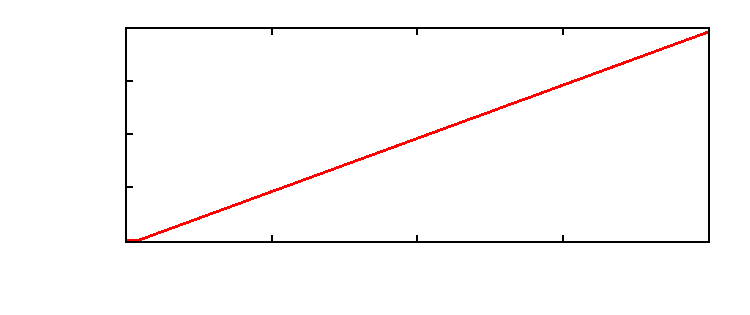
\includegraphics{esc/unstable_SC}}%
    \gplfronttext
  \end{picture}%
\endgroup
}
\caption{Backorder in the retailer for rolling horizon optimization
  without stability constraints.}
\label{fig:unstable_SC}
\end{figure*}
For a simple two-node supply chain, we have demonstrated that simply
reoptimizing an economic objective function at each time instance
could lead to undesirable closed loop performance. Although, we chose
a pathological cost function to demonstrate the undesirable closed
loop, for a more complex supply chain, it is difficult to apriori
analyze all the interactions and judge if the rolling horizon
optimization will yield a desirable closed-loop. Stability theory, on
the other hand, helps us design easily implementable online 
optimization problems that guarantee desirable closed-loop
properties. In Section \ref{sec:economicMPC_theory}, we outline the
stability theory for economic MPC and show that economic MPC
delivers a desirable closed loop, even for the pathological cost
function chosen in this section.

\subsection{Economic MPC theory}
\label{sec:economicMPC_theory}
\subsubsection{Terminal equality constraint formulation}
\label{subsec:terminal_equality}
In this section we outline the theory for economic MPC with terminal
equality constraint \citep{diehl:amrit:rawlings:2011} and economic MPC
with terminal penalty and region
\citep{amrit:rawlings:angeli:2011}. We only state the main
  assumptions and results here and refer the reader to the papers for
  details.
We consider the system given by \eqref{eq:model} expressed in the
state-space form $x^+=Ax+Bu+B_dd$. We consider the linear economic
cost given by \eqref{eq:ellE}. The states are constrained to lie in
the hyperbox $\underbar{x} \leq x \leq \bar{x}$ while the inputs lie in
$\underbar{u} \leq u \leq \bar{u}$ (The inequalities are
componentwise). We assume that the sets 
\[\mathbb{X}: \set{x \mid \underbar{x} \leq x \leq  \bar{x}} \qquad \mathbb{U}: \set{u \mid \underbar{u} \leq u \leq \bar{u}}\] are
bounded and contain the optimal steady-state defined later in
\eqref{eq:SS}.

Note that the choice of linear models and cost function automatically satisfies Assumption \ref{ass:cont}
stated below.

\begin{assumption}[Continuity]
\label{ass:cont}
The system and the stage costs are  continuous.
\end{assumption}

We define the steady-state optimization problem as follows:

\begin{align}
\label{eq:SS}
&\min_{x,u}{\ell_E(x,u;d_s)}  \nonumber \\ &\text{s.t~} x = Ax+Bu+B_dd, \\&x \in
\mathbb{X}, u \in \mathbb{U} \nonumber
\end{align}

We denote $(x_s,u_s;d_s)$ as the solution to \eqref{eq:SS} and make the
following assumptions on $(x_s,u_s;d_s)$. The nominal demand is
denoted as $d_s$.

\begin{assumption}[Strict dissipativity]
\label{ass:strict_dissipativity}
There exists $(x_s,u_s;d_s)$ and $\lambda_s$ so that 
\begin{enumerate}[(a)]
\item $(x_s,u_s;d_s)$  is an unique solution of \eqref{eq:SS}.
\item The multiplier $\lambda_s$ is such that $(x_s,u_s;d_s)$
  uniquely solves \eqref{eq:SS1}
\begin{equation}
\label{eq:SS1}
\min_{x,u}{\ell_E(x,u)+\lambda_s'[x-(Ax+Bu+B_dd_s)]-\ell_E(x_s,u_s)}
\end{equation}
\item The system $x^+=Ax+Bu+B_dd_s$ is strictly dissipative with respect
  to the supply rate $s(x,u) = \ell_E(x,u)-\ell_E(x_s,u_s)$ and
  storage function $\lambda(x) = \lambda_s'x$. That is, there exists a
  $\mathcal{K}_{\infty}$ function $\rho(\cdot)$ such that:
\begin{multline}
\label{eq:strict_dissipativity}
\lambda_s'(Ax+Bu+B_dd_s-x) \leq -\rho (x-x_s)+s(x,u),\\ \forall (x,u) \in
\mathbb{X} \times \mathbb{U}
\end{multline}
\end{enumerate}
\end{assumption}


Because of the structure of the state-space matrix $A$ in \eqref{eq:model}, the steady-state
problem \eqref{eq:SS} decomposes into two problems:
\begin{equation}
\label{eq:SSx} \min_{x}{q'x} \qquad \text{s.t~} \underbar{x} \leq x
\leq \bar{x}
\end{equation}
and
\begin{multline}
\label{eq:SSu} \min_{u}{r'u} \qquad \text{s.t~} B^{(1)}u + B^{(2)}u +
Bu + B_dd_s = 0,\\
 \underbar{u} \leq u\leq \bar{u}
\end{multline}

Since the set $\mathbb{X}$ is bounded, the solution to the first
optimization problem lies on one of the vertices of the hyperbox
defining $\mathbb{X}$. For instance, if all the elements of $q$ are
strictly positive, then $x_s = \underbar{x}$. Therefore, depending on
the input constraints, we can establish an unique steady-state for
$x$.

For the optimization
problem in $u$, we assume that the nominal disturbance $d_s$ is such
that the feasible space is not empty. Hence, the second linear program
also admits an unique solution when $\text{rank}(B^{(1)}+B^{(2)}+B)$ is $n$, with
$n$ being the dimension of the states ($x$). Controllability of the
state-space \eqref{eq:model} establishes that the rank condition is
satisfied. It is easy to show that centralized supply chain model is
controllable. Therefore, we have established that the
steady-state problem has an unique solution. By choosing $\lambda_s$
as the optimal Lagrange multiplier for the equality constraints in
\eqref{eq:SS}, we can establish that the $(x_s,u_s;d_s)$ is the unique
solution of optimization problem \eqref{eq:SS1}. 

{\em{todo:strict dissipativity of linear systems}}

Hence Assumption \ref{ass:strict_dissipativity} is satisfied by the
supply chain model.

We now define the terminal equality constraint MPC optimization
problem:
\begin{alignat}{1}
\label{eq:PT}
\mathbb{P}_T(x(k)):& \min_{\bu}{V(\bu;x(k),\bd,N)} \nonumber \\
&\text{s.t~} x(i+1) = Ax(i) + Bu(i)+B_dd(i), \nonumber\\
&\underbar{x} \leq x(i) \leq \bar{x},  \\
&\underbar{u} \leq u(i) \leq \bar{u}, \nonumber \\
&i = k,k+1,\ldots,k+N-1\nonumber\\
&x(k+N) = x_S \nonumber
\end{alignat}

in which $V(\bu;x(k),\bd,N) = \sum_{i=0}^{N-1}
\ell_E(x(k+i),u(k+i))$. Note that in contrast to problem \eqref{eq:P},
we have added a terminal constraint that $x(k+N) = x_s$ in problem
\eqref{eq:PT}. The terminal constraint ensures that the final state is
the steady-state obtained by the steady-state optimization problem
\eqref{eq:SS}.

Before presenting the stability theorem, attributed to
\citet{diehl:amrit:rawlings:2011}, we define the following sets and
the control law.

The set of admissible state-input pairs $(x,\bu)$ is denoted by
$\mathbb{Z}_T$ as follows:
\begin{multline*}\mathbb{Z}_T := \left \lbrace(x,\bu) \mid \phi(i;x,\bu,\bd_s) \in
  \mathbb{X} \right . ,\\ \left . \bu \in \mathbb{U}^N, \phi(N;x,\bu,\bd_s) = x_s\right\rbrace
\end{multline*}
in which $\bd_s$ is the nominal demand vector and
$\phi(i;x,\bu,\bd_s)$ denotes the solution at time $i$ under input
$\bu$ starting from $x$ at time $0$. 

The projection of set $\mathbb{Z}_T$ onto the feasible state space
$\mathbb{X}$ is called the set of admissible initial states,
$\mathcal{X}_{N,T}$

\[\mathcal{X}_{N,T} := \set{x \mid \exists \bu \in \mathbb{U}^N
  \text{s.t~} (x,\bu) \in \mathbb{Z}_T} \]

We denote the optimal solution of problem \eqref{eq:PT} as
$\bu^0(x(k),\bd_s)$. Denoting the first input in the sequence
$\bu^0(x(k),\bd_s)$ as $\kappa_T(x(k))$, we obtain the closed-loop
dynamics of the MPC algorithm as $x^+ = Ax+B\kappa_T(x)+B_dd_s$.  The
control law is $\kappa_T(x(k))$.

We also make the following assumption because we require some form of
system controllability
\begin{assumption}[Weak Controllability]
\label{ass:weak_controllability}
There exists a $\mathcal{K}_\infty$ function $\gamma(\cdot)$ such that
for every $x \in \mathcal{X}_{N,T}$, there exists $\bu$ such that
$(x,\bu) \in \mathbb{Z}_T$ and 
\begin{equation}
\label{eq:weak_controllability}
\sum_{i=0}^{N-1} \norm{u_i-u_s} \leq \gamma(\norm{x-x_s})
\end{equation}
\end{assumption}

Note that Assumption \ref{ass:weak_controllability} is satisfied by
linear stabilizable systems. Hence, it is satisfied for the supply
chain model.

\begin{theorem}[Lyapunov function with terminal equality constraint]
\label{thm:EqualityConstraint}
If Assumptions \ref{ass:cont} --- \ref{ass:weak_controllability}
hold, the steady-state solution of the closed-loop system $x^+ =
Ax+B\kappa_T(x)+B_dd_s$ is asymptotically stable with
$\mathcal{X}_{N,T}$ as the region of attraction. The Lyapunov function
is
\[ \tilde{V}(x) := V(x) +\lambda_s'[x-x_s]-N\ell_E(x_s,u_s) \]
\end{theorem}
 
Theorem \ref{thm:EqualityConstraint} allows us to conclude that
rolling horizon optimization in which we solve problem
$\mathbb{P}_T(x(k))$ at each sampling instance steer any initial state
$x(0) \in \mathcal{X}_{N,T}$ to the steady-state $x_s$. Therefore, in
contrast to the closed-loop observed in Figure \ref{fig:unstable_SC},
an MPC implementation minimizing $\mathbb{P}_T(x(k))$ would have never
left the steady-state, thereby only incurring a cost of $220$ per
period. In Figure \ref{fig:stable_SC}, we plot the closed-loop for a
$x(0) \neq x_s$ (using the same cost vector used in the previous
section).

\begin{figure*}
\centering
\scriptsize
\resizebox{\textwidth}{!}{% GNUPLOT: LaTeX picture with Postscript
\begingroup
  \makeatletter
  \providecommand\color[2][]{%
    \GenericError{(gnuplot) \space\space\space\@spaces}{%
      Package color not loaded in conjunction with
      terminal option `colourtext'%
    }{See the gnuplot documentation for explanation.%
    }{Either use 'blacktext' in gnuplot or load the package
      color.sty in LaTeX.}%
    \renewcommand\color[2][]{}%
  }%
  \providecommand\includegraphics[2][]{%
    \GenericError{(gnuplot) \space\space\space\@spaces}{%
      Package graphicx or graphics not loaded%
    }{See the gnuplot documentation for explanation.%
    }{The gnuplot epslatex terminal needs graphicx.sty or graphics.sty.}%
    \renewcommand\includegraphics[2][]{}%
  }%
  \providecommand\rotatebox[2]{#2}%
  \@ifundefined{ifGPcolor}{%
    \newif\ifGPcolor
    \GPcolorfalse
  }{}%
  \@ifundefined{ifGPblacktext}{%
    \newif\ifGPblacktext
    \GPblacktexttrue
  }{}%
  % define a \g@addto@macro without @ in the name:
  \let\gplgaddtomacro\g@addto@macro
  % define empty templates for all commands taking text:
  \gdef\gplbacktext{}%
  \gdef\gplfronttext{}%
  \makeatother
  \ifGPblacktext
    % no textcolor at all
    \def\colorrgb#1{}%
    \def\colorgray#1{}%
  \else
    % gray or color?
    \ifGPcolor
      \def\colorrgb#1{\color[rgb]{#1}}%
      \def\colorgray#1{\color[gray]{#1}}%
      \expandafter\def\csname LTw\endcsname{\color{white}}%
      \expandafter\def\csname LTb\endcsname{\color{black}}%
      \expandafter\def\csname LTa\endcsname{\color{black}}%
      \expandafter\def\csname LT0\endcsname{\color[rgb]{1,0,0}}%
      \expandafter\def\csname LT1\endcsname{\color[rgb]{0,1,0}}%
      \expandafter\def\csname LT2\endcsname{\color[rgb]{0,0,1}}%
      \expandafter\def\csname LT3\endcsname{\color[rgb]{1,0,1}}%
      \expandafter\def\csname LT4\endcsname{\color[rgb]{0,1,1}}%
      \expandafter\def\csname LT5\endcsname{\color[rgb]{1,1,0}}%
      \expandafter\def\csname LT6\endcsname{\color[rgb]{0,0,0}}%
      \expandafter\def\csname LT7\endcsname{\color[rgb]{1,0.3,0}}%
      \expandafter\def\csname LT8\endcsname{\color[rgb]{0.5,0.5,0.5}}%
    \else
      % gray
      \def\colorrgb#1{\color{black}}%
      \def\colorgray#1{\color[gray]{#1}}%
      \expandafter\def\csname LTw\endcsname{\color{white}}%
      \expandafter\def\csname LTb\endcsname{\color{black}}%
      \expandafter\def\csname LTa\endcsname{\color{black}}%
      \expandafter\def\csname LT0\endcsname{\color{black}}%
      \expandafter\def\csname LT1\endcsname{\color{black}}%
      \expandafter\def\csname LT2\endcsname{\color{black}}%
      \expandafter\def\csname LT3\endcsname{\color{black}}%
      \expandafter\def\csname LT4\endcsname{\color{black}}%
      \expandafter\def\csname LT5\endcsname{\color{black}}%
      \expandafter\def\csname LT6\endcsname{\color{black}}%
      \expandafter\def\csname LT7\endcsname{\color{black}}%
      \expandafter\def\csname LT8\endcsname{\color{black}}%
    \fi
  \fi
  \setlength{\unitlength}{0.0500bp}%
  \begin{picture}(7200.00,3024.00)%
    \gplgaddtomacro\gplbacktext{%
      \csname LTb\endcsname%
      \put(814,832){\makebox(0,0)[r]{\strut{} 0}}%
      \put(814,1475){\makebox(0,0)[r]{\strut{} 10}}%
      \put(814,2117){\makebox(0,0)[r]{\strut{} 20}}%
      \put(814,2759){\makebox(0,0)[r]{\strut{} 30}}%
      \put(946,484){\makebox(0,0){\strut{} 0}}%
      \put(1433,484){\makebox(0,0){\strut{} 2}}%
      \put(1921,484){\makebox(0,0){\strut{} 4}}%
      \put(2408,484){\makebox(0,0){\strut{} 6}}%
      \put(2896,484){\makebox(0,0){\strut{} 8}}%
      \put(3383,484){\makebox(0,0){\strut{} 10}}%
      \put(176,1731){\rotatebox{-270}{\makebox(0,0){\strut{}Inventory}}}%
      \put(2164,154){\makebox(0,0){\strut{}Time}}%
    }%
    \gplgaddtomacro\gplfronttext{%
      \csname LTb\endcsname%
      \put(2061,2970){\makebox(0,0)[r]{\strut{}Retailer}}%
    }%
    \gplgaddtomacro\gplbacktext{%
      \csname LTb\endcsname%
      \put(4109,484){\makebox(0,0){\strut{} 0}}%
      \put(4544,484){\makebox(0,0){\strut{} 2}}%
      \put(4978,484){\makebox(0,0){\strut{} 4}}%
      \put(5413,484){\makebox(0,0){\strut{} 6}}%
      \put(5847,484){\makebox(0,0){\strut{} 8}}%
      \put(6282,484){\makebox(0,0){\strut{} 10}}%
      \put(6414,998){\makebox(0,0)[l]{\strut{} 0}}%
      \put(6414,2465){\makebox(0,0)[l]{\strut{} 10}}%
      \put(7051,1731){\rotatebox{-270}{\makebox(0,0){\strut{}Backorder}}}%
      \put(5195,154){\makebox(0,0){\strut{}Time}}%
    }%
    \gplgaddtomacro\gplfronttext{%
      \csname LTb\endcsname%
      \put(5039,2943){\makebox(0,0)[r]{\strut{}Manufacturer}}%
    }%
    \gplbacktext
    \put(0,0){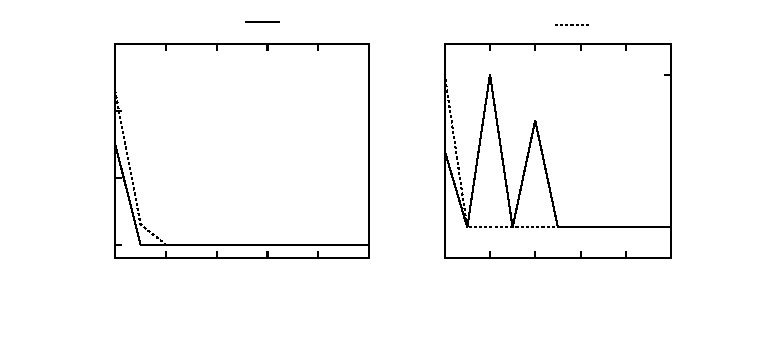
\includegraphics{stable_SC}}%
    \gplfronttext
  \end{picture}%
\endgroup
}
\caption{Closed loop evolution using stabilizing MPC.}
\label{fig:stable_SC}
\end{figure*}


Although economic MPC with terminal equality constraints stabilizes
the supply chain system, notice that the unique steady-state for the
states that is obtained by solving the linear program \eqref{eq:SSx}
is on one of the vertices of the hyperbox $\mathbb{X}$. More
importantly, since the cost vector $q$ is composed of inventory
holding and lost sales costs, all its elements are strictly
positive. Therefore, the solution of \eqref{eq:SSx} is $x_s =
\underbar{x}$. This steady-state value of the state variables has
an important implications which motivates us to formulate the
multiobjective supply chain MPC with terminal region in the next
section.

Supply chain managers often balance economic objectives with that of
risk minimization. That is, in addition to minimizing costs (or
maximizing profits), the manager also tries to minimize risk by
maintaining or by tracking inventory around a  safety-stock level
(that could determined by minimizing the probability of stock-out
etc. or is the solution of stochastic inventory control algorithms
like \citet{federgruen:1993, shang:song:2003, dong:lee:2003,
  gallego:ozer:2005,chen:song:2001}). As we stated above, stabilizing
economic-MPC can only stabilize $x_s = 0$ or $x_{\text{safety}}$, the
  safety-state. The safety state consists of $\Inv_{i,\text{safety}}$,
  the safety stock level for inventories and $0$, the target level for
  backorders. Since, practitioners consider the safety stock to be a
  soft constraint, we introduce a tracking stage cost \eqref{eq:ellT}
  and minimize a combined economic and tracking objective in the next section.

\subsubsection{Terminal region formulation}
\paragraph{Stage cost.} In order to allow the practitioner to implement
a controller that tracks inventories to a steady-state as well as
optimize the economics of the system, we use the following stage cost,
\begin{equation}
\label{eq:ell}
\ell(x,u) = \frac{\omega}{s_E} \ell_E(x,u) + \frac{(1-\omega)}{s_T} \ell_T(x,u;z_p)
\end{equation}
in which $\omega \in (0,1)$ is a relative weighting chosen by the
practitioner between the tracking and the economic stage costs. We use
the parameters $Q,R$ in $\ell_T(x,u)$ and $\omega$ as tuning
parameters for the multiobjective MPC controller. The parameters
$(s_E,s_T)$ are scaling constants while $z_p=(x_t,u_t)$ are the tracking
set-points.
\paragraph{Constraints.} The state constraint $x \in
\mathbb{X}$ consists of upper bounds on inventory and backorders
$\bar{x}$ and non-negativity of inventory and backorders
$\underbar{x}=0$. As in the previous section,  $ u \in \mathbb{U} := \set{u \mid \underbar{u} \leq
  u \leq \bar{u}}$.



\paragraph{Steady-state.}
We choose the input target $u_t$ to be the ``economic'' input that
satisfies the nominal demand, that is $u_t = u_s$ in which $u_s$ is
the solution to \eqref{eq:SSu}. The target set-point for the states is
$x_t = x_{\text{safety}}$. The steady-state optimization problem
now becomes
\begin{align}
\label{eq:SSMulti}
&\min_{x,u}{}(\frac{\omega}{s_E} (q'x+r'u) + \nonumber\\
&\frac{(1-\omega)}{s_T}((x-x_{\text{safety}})'Q(x-x_{\text{safety}})+(u-u_s)'R(u-u_s)))\\
&\text{s.t~} x=Ax+Bu+B_dd_s, u \in \mathbb{U}, x \in \mathbb{X} \nonumber\\
\end{align}

To obtain the scaling parameters $s_T,s_E$, we consider the utopia and
nadir points of the individual stage costs $\ell_E(x,u)$ and
$\ell_T(x,u;z_p)$. Denoting $z = (x,u)$, we obtain
\[ z_E = \text{arg}\min_{z \in \mathbb{X} \times
  \mathbb{U}}{\ell_E(x,u)}, \quad z_T = \text{arg}\min_{z \in \mathbb{X} \times
  \mathbb{U}}{\ell_T(x,u;z_p)} \]

The utopia point is $J^U = (\ell_E(z_E),\ell_T(z_T;z_p))\in \mathbb{R}^2$. The
nadir point is $J^N = (\ell_E(z_T),\ell_T(z_E;z_p))$. The parameters
$s_T,s_E$ are then defined as:
\[ (s_E,s_T) = J^N-J^U \]

Note that  the optimization problem \eqref{eq:SSMulti} is a quadratic program with a positive
definite Hessian, and hence an unique solution to \eqref{eq:SSMulti}
exists.
The solution to \eqref{eq:SSMulti}, $x_s,u_s$,  is unique for a given
choice of $(\omega,x_t,u_t)$ and only depends on $d_s$ and
the cost vector $r$. Therefore, based on the choice $\omega$ and
tuning parameters $(Q,R)$, the MPC controller described in this section stabilizes a different
$x_s$. That is, the choice of weighting given to the economic and
tracking objectives decide what levels the controller is going to stabilize.


In Figure \ref{fig:SS_omega}, we plot the inventory steady-state as a
function of $\omega$. The parameters used are $ Q =
10\diag{(1,1,1,1)}, R = 10^{-5}\diag{(1,1,1,1)}$, $x_{\text{safety}}
= (35,0,40,0)$. The economic costs are $q = (10,10,10,1), r =
(10,0.1,10,100)$. The input and state constraints were chosen as
\[ 0 \leq x \leq 100 \qquad 0 \leq u \leq 20 \]
The nominal demand
$d_s$ was $10$. Note that by choice of the state targets,the
steady-state backorders at both nodes is zero.

\begin{figure*}
\centering
\scriptsize
\resizebox{\textwidth}{!}{% GNUPLOT: LaTeX picture with Postscript
\begingroup
  \makeatletter
  \providecommand\color[2][]{%
    \GenericError{(gnuplot) \space\space\space\@spaces}{%
      Package color not loaded in conjunction with
      terminal option `colourtext'%
    }{See the gnuplot documentation for explanation.%
    }{Either use 'blacktext' in gnuplot or load the package
      color.sty in LaTeX.}%
    \renewcommand\color[2][]{}%
  }%
  \providecommand\includegraphics[2][]{%
    \GenericError{(gnuplot) \space\space\space\@spaces}{%
      Package graphicx or graphics not loaded%
    }{See the gnuplot documentation for explanation.%
    }{The gnuplot epslatex terminal needs graphicx.sty or graphics.sty.}%
    \renewcommand\includegraphics[2][]{}%
  }%
  \providecommand\rotatebox[2]{#2}%
  \@ifundefined{ifGPcolor}{%
    \newif\ifGPcolor
    \GPcolortrue
  }{}%
  \@ifundefined{ifGPblacktext}{%
    \newif\ifGPblacktext
    \GPblacktexttrue
  }{}%
  % define a \g@addto@macro without @ in the name:
  \let\gplgaddtomacro\g@addto@macro
  % define empty templates for all commands taking text:
  \gdef\gplbacktext{}%
  \gdef\gplfronttext{}%
  \makeatother
  \ifGPblacktext
    % no textcolor at all
    \def\colorrgb#1{}%
    \def\colorgray#1{}%
  \else
    % gray or color?
    \ifGPcolor
      \def\colorrgb#1{\color[rgb]{#1}}%
      \def\colorgray#1{\color[gray]{#1}}%
      \expandafter\def\csname LTw\endcsname{\color{white}}%
      \expandafter\def\csname LTb\endcsname{\color{black}}%
      \expandafter\def\csname LTa\endcsname{\color{black}}%
      \expandafter\def\csname LT0\endcsname{\color[rgb]{1,0,0}}%
      \expandafter\def\csname LT1\endcsname{\color[rgb]{0,1,0}}%
      \expandafter\def\csname LT2\endcsname{\color[rgb]{0,0,1}}%
      \expandafter\def\csname LT3\endcsname{\color[rgb]{1,0,1}}%
      \expandafter\def\csname LT4\endcsname{\color[rgb]{0,1,1}}%
      \expandafter\def\csname LT5\endcsname{\color[rgb]{1,1,0}}%
      \expandafter\def\csname LT6\endcsname{\color[rgb]{0,0,0}}%
      \expandafter\def\csname LT7\endcsname{\color[rgb]{1,0.3,0}}%
      \expandafter\def\csname LT8\endcsname{\color[rgb]{0.5,0.5,0.5}}%
    \else
      % gray
      \def\colorrgb#1{\color{black}}%
      \def\colorgray#1{\color[gray]{#1}}%
      \expandafter\def\csname LTw\endcsname{\color{white}}%
      \expandafter\def\csname LTb\endcsname{\color{black}}%
      \expandafter\def\csname LTa\endcsname{\color{black}}%
      \expandafter\def\csname LT0\endcsname{\color{black}}%
      \expandafter\def\csname LT1\endcsname{\color{black}}%
      \expandafter\def\csname LT2\endcsname{\color{black}}%
      \expandafter\def\csname LT3\endcsname{\color{black}}%
      \expandafter\def\csname LT4\endcsname{\color{black}}%
      \expandafter\def\csname LT5\endcsname{\color{black}}%
      \expandafter\def\csname LT6\endcsname{\color{black}}%
      \expandafter\def\csname LT7\endcsname{\color{black}}%
      \expandafter\def\csname LT8\endcsname{\color{black}}%
    \fi
  \fi
  \setlength{\unitlength}{0.0500bp}%
  \begin{picture}(7200.00,3024.00)%
    \gplgaddtomacro\gplbacktext{%
      \csname LTb\endcsname%
      \put(814,802){\makebox(0,0)[r]{\strut{} 0}}%
      \put(814,1291){\makebox(0,0)[r]{\strut{} 10}}%
      \put(814,1780){\makebox(0,0)[r]{\strut{} 20}}%
      \put(814,2270){\makebox(0,0)[r]{\strut{} 30}}%
      \put(814,2759){\makebox(0,0)[r]{\strut{} 40}}%
      \put(946,484){\makebox(0,0){\strut{} 0}}%
      \put(3383,484){\makebox(0,0){\strut{} 1}}%
      \put(176,1731){\rotatebox{-270}{\makebox(0,0){\strut{}Inventory}}}%
      \put(2164,154){\makebox(0,0){\strut{}$\omega$}}%
    }%
    \gplgaddtomacro\gplfronttext{%
      \csname LTb\endcsname%
      \put(2396,2586){\makebox(0,0)[r]{\strut{}Retailer}}%
    }%
    \gplgaddtomacro\gplbacktext{%
      \csname LTb\endcsname%
      \put(4109,484){\makebox(0,0){\strut{} 0}}%
      \put(6282,484){\makebox(0,0){\strut{} 1}}%
      \put(6414,791){\makebox(0,0)[l]{\strut{} 0}}%
      \put(6414,1229){\makebox(0,0)[l]{\strut{} 10}}%
      \put(6414,1666){\makebox(0,0)[l]{\strut{} 20}}%
      \put(6414,2103){\makebox(0,0)[l]{\strut{} 30}}%
      \put(6414,2540){\makebox(0,0)[l]{\strut{} 40}}%
      \put(7051,1731){\rotatebox{-270}{\makebox(0,0){\strut{}Inventory}}}%
      \put(5195,154){\makebox(0,0){\strut{}$\omega$}}%
    }%
    \gplgaddtomacro\gplfronttext{%
      \csname LTb\endcsname%
      \put(5295,2586){\makebox(0,0)[r]{\strut{}Manufacturer}}%
    }%
    \gplbacktext
    \put(0,0){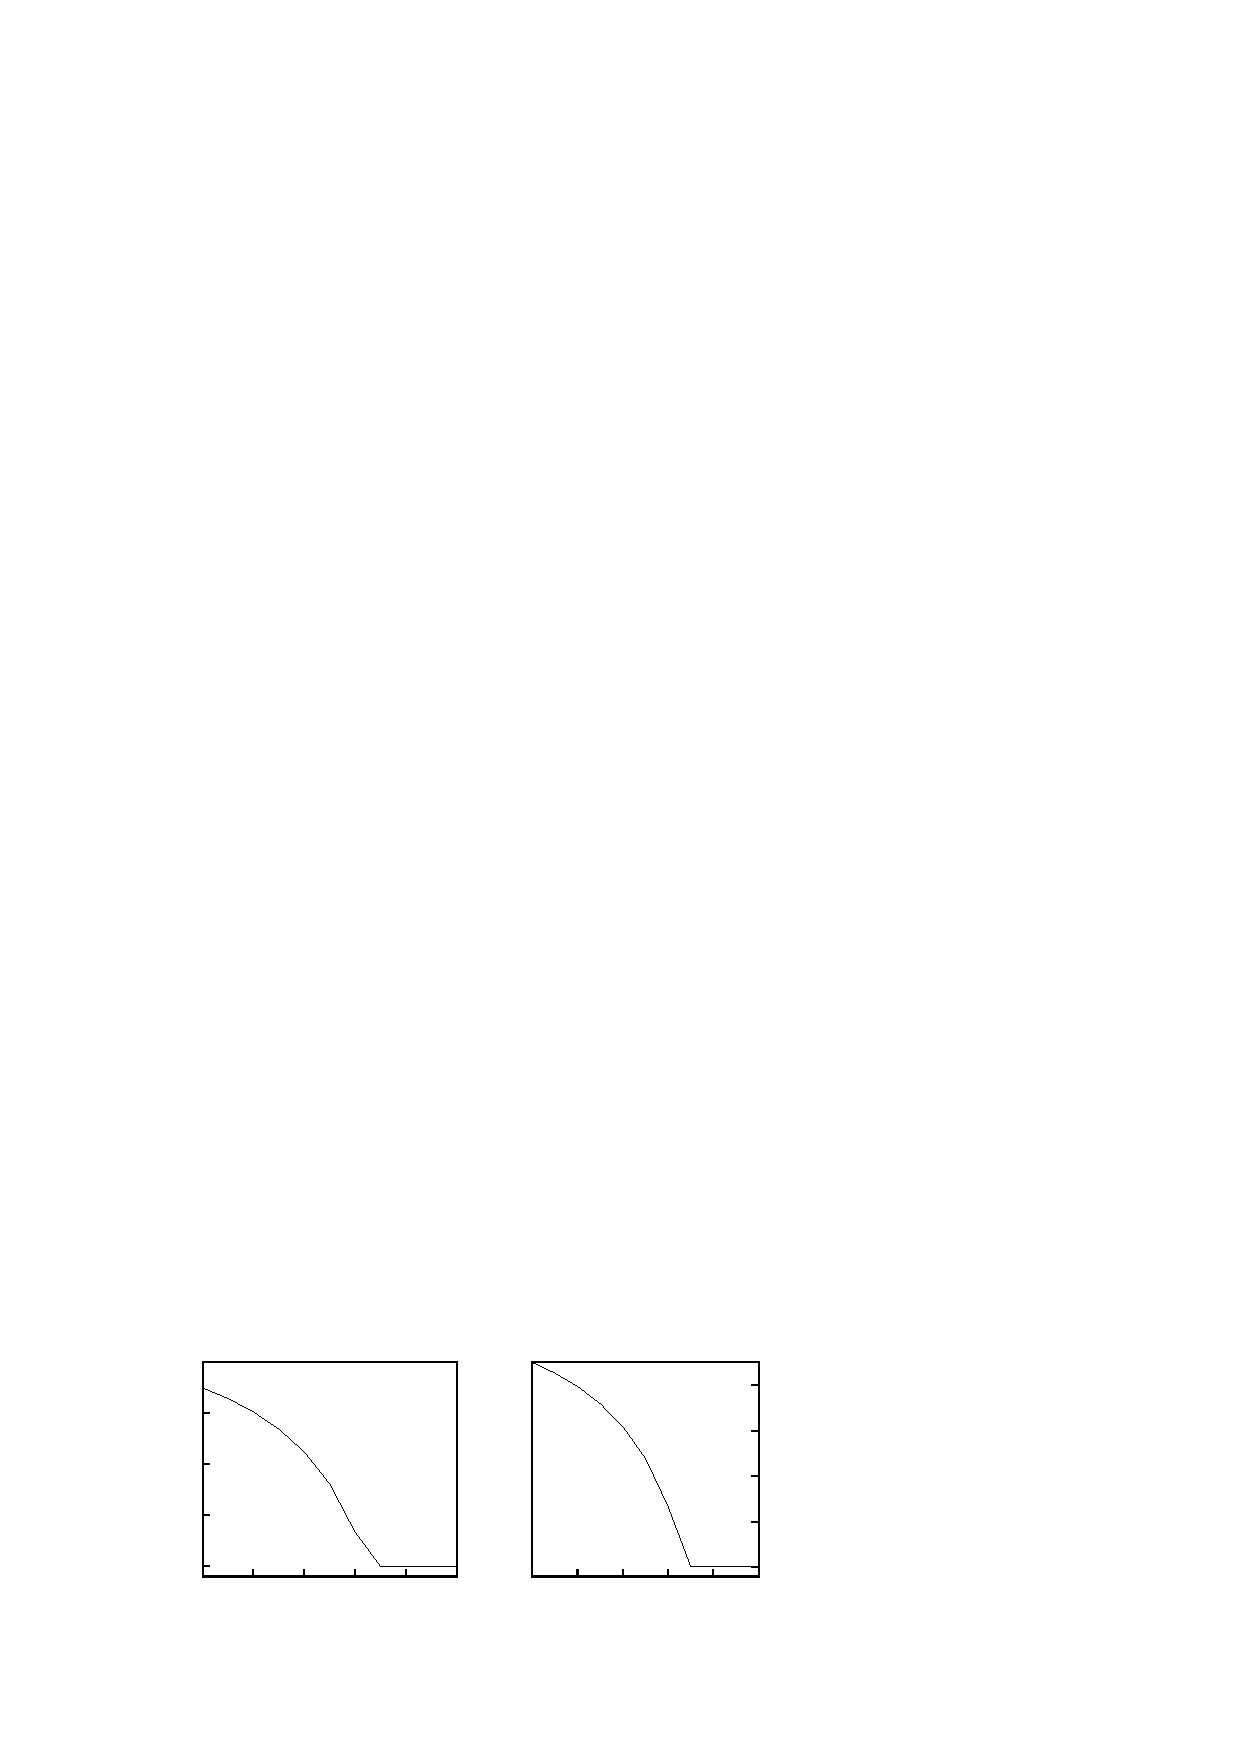
\includegraphics{esc/SS_omega}}%
    \gplfronttext
  \end{picture}%
\endgroup
}
\caption{Steady-state as a function of the relative weighting between tracking and
  economics}
\label{fig:SS_omega}
\end{figure*}

Figure \ref{fig:SS_omega} shows the trade-off between choosing to
track to the safety stock and choosing to minimize the economics. As
the economic weighting is increased, we see that the steady-state
approaches the economic steady-state.

\paragraph{Terminal region and Terminal penalty.}
Let  Assumptions \ref{ass:cont} and
\ref{ass:strict_dissipativity}(a) and
\ref{ass:strict_dissipativity}(c) hold. In Assumption
\ref{ass:strict_dissipativity}, we use $\ell(x,u)-\ell(x_s,u_s)$ in
which $\ell(x,u)$ is given by \eqref{eq:ell} and $(x_s,u_s)$ is the
solution of the steady-state problem \eqref{eq:SSMulti} as the storage
function. In addition, we make the following assumption:

\begin{assumption}[Basic stability assumption]
\label{ass:BSA}
There exists a compact terminal region $\mathbb{X}_f \subseteq
\mathbb{X}$, containing the point $x_s$ in its interior and a control
law $\kappa_f: \mathbb{X}_f \rightarrow \mathbb{U}$  and a function
$V_f:\mathbb{X}_f \rightarrow \mathbb{R}$ such that the
following holds
\begin{align}
\label{eq:BSA}
V_f(Ax+B\kappa_f(x)+B_dd_s) &\leq \nonumber\\
V_f(x)-\ell(x,\kappa_f(x))+\ell(x_s,u_s),& \\
&\forall x \in \mathbb{X}_f \nonumber \\
\label{eq:invariant}
Ax+ B\kappa_f(x) +B_dd_s \in \mathbb{X}_f&, \\ & \forall x \in
\mathbb{X}_f \nonumber
\end{align}
\end{assumption}

We now define the terminal penalty MPC problem:
\begin{alignat}{1}
\label{eq:PP}
\mathbb{P}_P(x(k)):& \min_{\bu}{V(\bu;x(k),\bd,N)} \nonumber \\
&\text{s.t~} x(i+1) = Ax(i) + Bu(i)+B_dd(i), \nonumber\\
&\underbar{x} \leq x(i) \leq \bar{x},  \\
&\underbar{u} \leq u(i) \leq \bar{u}, \nonumber \\
&i = k,k+1,\ldots,k+N-1\nonumber\\
&x(k+N) \in \mathbb{X}_f \nonumber
\end{alignat}

in which $V_P(\bu;x(k),\bd_s,N) = \sum_{i=0}^{N-1}
\ell(x(k+i),u(k+i))+ V_f(x(k+N))$.

Note the two differences between terminal equality constraint problem
$\mathbb{P}_T$ and the terminal penalty formulation $\mathbb{P}_P$:
(i) The constraint $x(k+N) = x_S$ is replaced by $x(k+N) \in
\mathbb{X}_f$ and (ii) The objective function is $V_P(\bu;x(k),\bd_s,N) =
V(\bu;x(k),\bu,N) + V_f(x(k+N))$, that is, a terminal penalty is added
to the objective function. 

Analogous to $\mathbb{Z}_T$ and $\mathcal{X}_{N,T}$, we define the
sets $\mathbb{Z}_P$ and $\mathbb{X}_{N,P}$ (the subscript $P$ refers
to terminal penalty) as follows:
\[ \mathbb{Z}_P := \set{(x,\bu) \mid  \bu \in \mathbb{U}^N,
  \phi(N;x,\bu,\bd_s) \in \mathbb{X}_f}\]
in which $\bd_s$ is the nominal demand vector and
$\phi(i;x,\bu,\bd_s)$ denotes the solution at time $i$ under input
$\bu$ starting from $x$ at time $0$. 

The projection of set $\mathbb{Z}_P$ onto the feasible state space
$\mathbb{X}$ is called the set of admissible initial states,
$\mathcal{X}_{N,P}$


\[\mathcal{X}_{N,P} := \set{x \mid \exists \bu \in \mathbb{U}^N
  \text{s.t~} (x,\bu) \in \mathbb{Z}_P} \]

We denote the optimal solution of problem \eqref{eq:PP} as
$\bu^0(x(k),\bd_s)$. Denoting the first input in the sequence
$\bu^0(x(k),\bd_s)$ as $\kappa_P(x(k))$, we obtain the closed-loop
dynamics of the MPC algorithm as $x^+ = Ax+B\kappa_P(x)+B_dd_s$.  The
control law is $\kappa_P(x(k))$.

To show that the closed-loop using the control law $u = \kappa_P(x)$
is asymptotically stable, we need to make the following  assumption:

\begin{assumption}[Continuity of the storage function]
\label{ass:cont_lambda}
The storage function $\lambda(\cdot)$ is continuous on $\mathbb{X}
\times  \mathbb{U}$
\end{assumption}

The following theorem attributed to \citet{amrit:rawlings:angeli:2011}
establishes that the closed-loop $x^+ = Ax+B\kappa_P(x)+B_dd_s$ is
asymptotically stable.

\begin{theorem}[Lyapunov stability with terminal region]
Let Assumptions \ref{ass:cont}, \ref{ass:strict_dissipativity}(a),
\ref{ass:strict_dissipativity}(c), \ref{ass:BSA} and
\ref{ass:cont_lambda} hold. Then the steady-state solution $x_s$ is an
asymptotically stable equilibrium point of the system
$x^+=Ax+B\kappa_P(x)+B_dd_s$ with the region of attraction being any
arbitrarily large compact subset of $\mathcal{X}_{N,P}$. The Lyapunov
function is \begin{multline*}\bar{V}_P^0(\bu;x(k),\bd_s,N) =
V_P^0(\bu;x(k),\bd_s,N)\\-N\ell(x_s,u_s)-\lambda(x_s)-V_f(x_s)\end{multline*} in which
$V_P^0(\bu;x(k),\bd_s,N)$ is the optimal value function in the solution
of problem \eqref{eq:PP}.
\end{theorem}

We now discuss the choice of terminal region and terminal penalty for
the supply chain model. Note that the optimal Lagrange multiplier for
the equality constraints in steady-state problem \eqref{eq:SSMulti}
satisfies all the requirements in Assumptions
\ref{ass:strict_dissipativity} and \ref{ass:cont_lambda}. 

For the supply chain model, we choose the terminal controller
$\kappa_f(x) = Kx$, in which the gain $K$ is such that $A_K :=A+BK$ is
a Hurwitz. That is, the system $\tilde{x}^+ = A_K\tilde{x}$ is
asymptotically stable with the equilibrium point being $x_s$, in
which $\tilde{x}$ is the deviation variable $x-x_s$. Note that the
input is $\tilde{u} = K\tilde{x}$.  Since the supply
chain model $(A,B)$ is stabilizable, such an $K$ exists (for example,
the infinite horizon unconstrained LQR gain). By the choice
$\underbar{x} = 0$  and backorder targets, some state constraints are
active at the steady state. Hence,  we find $K$ using the technique given by
\citet{rao:rawlings:1999}. By this choice of the controller gain, we
restrict the evolution of the closed-loop $(A+BK)\tilde{x}$ to the
null space of the active constraints at the origin (the steady state
is shifted to the origin in deviation variables). We define $Q_K = Q+K'RK$
and $q_K = q+K'r$. We choose the terminal penalty to be 
\begin{equation}
\label{eq:Vf}
V_f(x;x_s) = (x-x_s)'P(x-x_s)+ p'(x-x_s)
\end{equation}

in which the positive definite matrix $P$ is the solution to the
Lyapunov equation
\[ A_K'PA_K-P = -Q_K \]
and $p$ is the solution to 
\[ (A_K-I)'p = -q_K \]

In order that the basic stability assumption be satisfied, we require
that  
\begin{equation}
\label{eq:BSA_condition}
(x-x_s)'Q(x_s-x_t)  \leq 0
\end{equation}


Therefore, we construct the terminal region $\mathbb{X}_f$ as the
following set:
\begin{multline}
\label{eq:Xf}
\mathbb{X}_f := \left \lbrace x \mid A_Kx+Bu_s+B_dd_s \in
  \mathbb{X}_f, \right. \\ \left.
  K(x-x_s)+u_s \in \mathbb{U}, (x-x_s)'Q(x_s-x_t) \leq 0\right \rbrace
\end{multline}

Such a set can be constructed using the maximal output admissible set
algorithm presented in \citet{gilbert:tan:1991} or by using the
efficient algorithms presented in the MPT toolbox
\citep{kvasnica:grieder:baotic:2006}. In Figure \ref{fig:Xf4}, we plot
the projection of the terminal region on the $\Inv_1-\Inv_2$
plane. The cost functions and constraints were the same as in the
steady-state calculation. The parameter $\omega$ is chosen to be
$0.4$.

\begin{figure*}
\centering
\scriptsize
\resizebox{0.75\textwidth}{!}{% GNUPLOT: LaTeX picture with Postscript
\begingroup
  \makeatletter
  \providecommand\color[2][]{%
    \GenericError{(gnuplot) \space\space\space\@spaces}{%
      Package color not loaded in conjunction with
      terminal option `colourtext'%
    }{See the gnuplot documentation for explanation.%
    }{Either use 'blacktext' in gnuplot or load the package
      color.sty in LaTeX.}%
    \renewcommand\color[2][]{}%
  }%
  \providecommand\includegraphics[2][]{%
    \GenericError{(gnuplot) \space\space\space\@spaces}{%
      Package graphicx or graphics not loaded%
    }{See the gnuplot documentation for explanation.%
    }{The gnuplot epslatex terminal needs graphicx.sty or graphics.sty.}%
    \renewcommand\includegraphics[2][]{}%
  }%
  \providecommand\rotatebox[2]{#2}%
  \@ifundefined{ifGPcolor}{%
    \newif\ifGPcolor
    \GPcolortrue
  }{}%
  \@ifundefined{ifGPblacktext}{%
    \newif\ifGPblacktext
    \GPblacktexttrue
  }{}%
  % define a \g@addto@macro without @ in the name:
  \let\gplgaddtomacro\g@addto@macro
  % define empty templates for all commands taking text:
  \gdef\gplbacktext{}%
  \gdef\gplfronttext{}%
  \makeatother
  \ifGPblacktext
    % no textcolor at all
    \def\colorrgb#1{}%
    \def\colorgray#1{}%
  \else
    % gray or color?
    \ifGPcolor
      \def\colorrgb#1{\color[rgb]{#1}}%
      \def\colorgray#1{\color[gray]{#1}}%
      \expandafter\def\csname LTw\endcsname{\color{white}}%
      \expandafter\def\csname LTb\endcsname{\color{black}}%
      \expandafter\def\csname LTa\endcsname{\color{black}}%
      \expandafter\def\csname LT0\endcsname{\color[rgb]{1,0,0}}%
      \expandafter\def\csname LT1\endcsname{\color[rgb]{0,1,0}}%
      \expandafter\def\csname LT2\endcsname{\color[rgb]{0,0,1}}%
      \expandafter\def\csname LT3\endcsname{\color[rgb]{1,0,1}}%
      \expandafter\def\csname LT4\endcsname{\color[rgb]{0,1,1}}%
      \expandafter\def\csname LT5\endcsname{\color[rgb]{1,1,0}}%
      \expandafter\def\csname LT6\endcsname{\color[rgb]{0,0,0}}%
      \expandafter\def\csname LT7\endcsname{\color[rgb]{1,0.3,0}}%
      \expandafter\def\csname LT8\endcsname{\color[rgb]{0.5,0.5,0.5}}%
    \else
      % gray
      \def\colorrgb#1{\color{black}}%
      \def\colorgray#1{\color[gray]{#1}}%
      \expandafter\def\csname LTw\endcsname{\color{white}}%
      \expandafter\def\csname LTb\endcsname{\color{black}}%
      \expandafter\def\csname LTa\endcsname{\color{black}}%
      \expandafter\def\csname LT0\endcsname{\color{black}}%
      \expandafter\def\csname LT1\endcsname{\color{black}}%
      \expandafter\def\csname LT2\endcsname{\color{black}}%
      \expandafter\def\csname LT3\endcsname{\color{black}}%
      \expandafter\def\csname LT4\endcsname{\color{black}}%
      \expandafter\def\csname LT5\endcsname{\color{black}}%
      \expandafter\def\csname LT6\endcsname{\color{black}}%
      \expandafter\def\csname LT7\endcsname{\color{black}}%
      \expandafter\def\csname LT8\endcsname{\color{black}}%
    \fi
  \fi
  \setlength{\unitlength}{0.0500bp}%
  \begin{picture}(7200.00,5040.00)%
    \gplgaddtomacro\gplbacktext{%
      \csname LTb\endcsname%
      \put(814,704){\makebox(0,0)[r]{\strut{} 0}}%
      \put(814,1383){\makebox(0,0)[r]{\strut{} 10}}%
      \put(814,2061){\makebox(0,0)[r]{\strut{} 20}}%
      \put(814,2740){\makebox(0,0)[r]{\strut{} 30}}%
      \put(814,3418){\makebox(0,0)[r]{\strut{} 40}}%
      \put(814,4097){\makebox(0,0)[r]{\strut{} 50}}%
      \put(814,4775){\makebox(0,0)[r]{\strut{} 60}}%
      \put(946,484){\makebox(0,0){\strut{} 0}}%
      \put(1678,484){\makebox(0,0){\strut{} 10}}%
      \put(2410,484){\makebox(0,0){\strut{} 20}}%
      \put(3142,484){\makebox(0,0){\strut{} 30}}%
      \put(3875,484){\makebox(0,0){\strut{} 40}}%
      \put(4607,484){\makebox(0,0){\strut{} 50}}%
      \put(5339,484){\makebox(0,0){\strut{} 60}}%
      \put(6071,484){\makebox(0,0){\strut{} 70}}%
      \put(6803,484){\makebox(0,0){\strut{} 80}}%
      \put(176,2739){\rotatebox{-270}{\makebox(0,0){\strut{}Inventory-Manufacturer}}}%
      \put(3874,154){\makebox(0,0){\strut{}Inventory-Retailer}}%
    }%
    \gplgaddtomacro\gplfronttext{%
    }%
    \gplbacktext
    \put(0,0){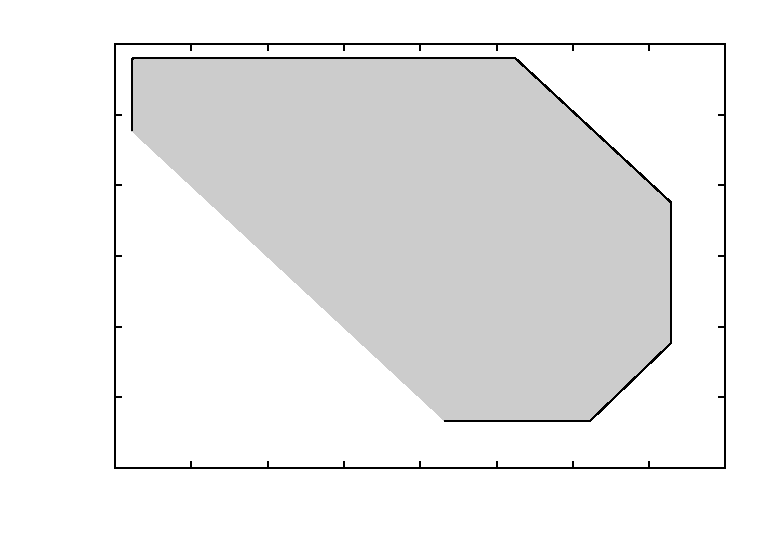
\includegraphics{esc/Xf4}}%
    \gplfronttext
  \end{picture}%
\endgroup
}
\caption{Projection of the terminal region onto the Inventory-plane
  for $\omega = 0.4$}
\label{fig:Xf4}
\end{figure*}


In Figure \ref{fig:CL}, we plot the closed-loop response for different
values of $\omega$. We contrast the performance to a pure tracking-MPC
that tracks to the steady-state solution of the multiobjective
formulation using $\ell(x,u;z_p)$ as the stage cost. That is, we
compare the closed-loop from solving problem \eqref{eq:PP} with the
closed-loop for $\omega = 0$ and $z_p = z_s$. Note that, from the
initial condition we chose $x(0) = (15,10,23,0)$, economic-MPC that
tracks to $z_s$ is only feasible for $\omega < 0.6$ (since we need
that $x_s \leq x(0)$).  

\begin{figure*}
\centering
\scriptsize
\resizebox{\textwidth}{!}{% GNUPLOT: LaTeX picture with Postscript
\begingroup
  \makeatletter
  \providecommand\color[2][]{%
    \GenericError{(gnuplot) \space\space\space\@spaces}{%
      Package color not loaded in conjunction with
      terminal option `colourtext'%
    }{See the gnuplot documentation for explanation.%
    }{Either use 'blacktext' in gnuplot or load the package
      color.sty in LaTeX.}%
    \renewcommand\color[2][]{}%
  }%
  \providecommand\includegraphics[2][]{%
    \GenericError{(gnuplot) \space\space\space\@spaces}{%
      Package graphicx or graphics not loaded%
    }{See the gnuplot documentation for explanation.%
    }{The gnuplot epslatex terminal needs graphicx.sty or graphics.sty.}%
    \renewcommand\includegraphics[2][]{}%
  }%
  \providecommand\rotatebox[2]{#2}%
  \@ifundefined{ifGPcolor}{%
    \newif\ifGPcolor
    \GPcolortrue
  }{}%
  \@ifundefined{ifGPblacktext}{%
    \newif\ifGPblacktext
    \GPblacktexttrue
  }{}%
  % define a \g@addto@macro without @ in the name:
  \let\gplgaddtomacro\g@addto@macro
  % define empty templates for all commands taking text:
  \gdef\gplbacktext{}%
  \gdef\gplfronttext{}%
  \makeatother
  \ifGPblacktext
    % no textcolor at all
    \def\colorrgb#1{}%
    \def\colorgray#1{}%
  \else
    % gray or color?
    \ifGPcolor
      \def\colorrgb#1{\color[rgb]{#1}}%
      \def\colorgray#1{\color[gray]{#1}}%
      \expandafter\def\csname LTw\endcsname{\color{white}}%
      \expandafter\def\csname LTb\endcsname{\color{black}}%
      \expandafter\def\csname LTa\endcsname{\color{black}}%
      \expandafter\def\csname LT0\endcsname{\color[rgb]{1,0,0}}%
      \expandafter\def\csname LT1\endcsname{\color[rgb]{0,1,0}}%
      \expandafter\def\csname LT2\endcsname{\color[rgb]{0,0,1}}%
      \expandafter\def\csname LT3\endcsname{\color[rgb]{1,0,1}}%
      \expandafter\def\csname LT4\endcsname{\color[rgb]{0,1,1}}%
      \expandafter\def\csname LT5\endcsname{\color[rgb]{1,1,0}}%
      \expandafter\def\csname LT6\endcsname{\color[rgb]{0,0,0}}%
      \expandafter\def\csname LT7\endcsname{\color[rgb]{1,0.3,0}}%
      \expandafter\def\csname LT8\endcsname{\color[rgb]{0.5,0.5,0.5}}%
    \else
      % gray
      \def\colorrgb#1{\color{black}}%
      \def\colorgray#1{\color[gray]{#1}}%
      \expandafter\def\csname LTw\endcsname{\color{white}}%
      \expandafter\def\csname LTb\endcsname{\color{black}}%
      \expandafter\def\csname LTa\endcsname{\color{black}}%
      \expandafter\def\csname LT0\endcsname{\color{black}}%
      \expandafter\def\csname LT1\endcsname{\color{black}}%
      \expandafter\def\csname LT2\endcsname{\color{black}}%
      \expandafter\def\csname LT3\endcsname{\color{black}}%
      \expandafter\def\csname LT4\endcsname{\color{black}}%
      \expandafter\def\csname LT5\endcsname{\color{black}}%
      \expandafter\def\csname LT6\endcsname{\color{black}}%
      \expandafter\def\csname LT7\endcsname{\color{black}}%
      \expandafter\def\csname LT8\endcsname{\color{black}}%
    \fi
  \fi
  \setlength{\unitlength}{0.0500bp}%
  \begin{picture}(7200.00,3024.00)%
    \gplgaddtomacro\gplbacktext{%
      \csname LTb\endcsname%
      \put(814,704){\makebox(0,0)[r]{\strut{} 10}}%
      \put(814,1389){\makebox(0,0)[r]{\strut{} 20}}%
      \put(814,2074){\makebox(0,0)[r]{\strut{} 30}}%
      \put(814,2759){\makebox(0,0)[r]{\strut{} 40}}%
      \put(946,484){\makebox(0,0){\strut{} 0}}%
      \put(2898,484){\makebox(0,0){\strut{} 10}}%
      \put(4851,484){\makebox(0,0){\strut{} 20}}%
      \put(6803,484){\makebox(0,0){\strut{} 30}}%
      \put(176,1731){\rotatebox{-270}{\makebox(0,0){\strut{}Inventory at Retailer}}}%
      \put(3874,154){\makebox(0,0){\strut{}Time}}%
      \put(4851,1732){\makebox(0,0)[l]{\strut{}Nominal state reset}}%
    }%
    \gplgaddtomacro\gplfronttext{%
      \csname LTb\endcsname%
      \put(4037,877){\makebox(0,0)[r]{\strut{}Actual}}%
      \csname LTb\endcsname%
      \put(5816,877){\makebox(0,0)[r]{\strut{}Nominal}}%
    }%
    \gplbacktext
    \put(0,0){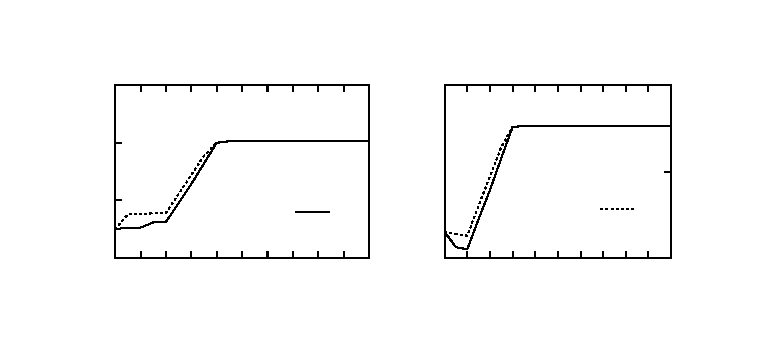
\includegraphics{CL2}}%
    \gplfronttext
  \end{picture}%
\endgroup
}
\resizebox{\textwidth}{!}{% GNUPLOT: LaTeX picture with Postscript
\begingroup
  \makeatletter
  \providecommand\color[2][]{%
    \GenericError{(gnuplot) \space\space\space\@spaces}{%
      Package color not loaded in conjunction with
      terminal option `colourtext'%
    }{See the gnuplot documentation for explanation.%
    }{Either use 'blacktext' in gnuplot or load the package
      color.sty in LaTeX.}%
    \renewcommand\color[2][]{}%
  }%
  \providecommand\includegraphics[2][]{%
    \GenericError{(gnuplot) \space\space\space\@spaces}{%
      Package graphicx or graphics not loaded%
    }{See the gnuplot documentation for explanation.%
    }{The gnuplot epslatex terminal needs graphicx.sty or graphics.sty.}%
    \renewcommand\includegraphics[2][]{}%
  }%
  \providecommand\rotatebox[2]{#2}%
  \@ifundefined{ifGPcolor}{%
    \newif\ifGPcolor
    \GPcolortrue
  }{}%
  \@ifundefined{ifGPblacktext}{%
    \newif\ifGPblacktext
    \GPblacktexttrue
  }{}%
  % define a \g@addto@macro without @ in the name:
  \let\gplgaddtomacro\g@addto@macro
  % define empty templates for all commands taking text:
  \gdef\gplbacktext{}%
  \gdef\gplfronttext{}%
  \makeatother
  \ifGPblacktext
    % no textcolor at all
    \def\colorrgb#1{}%
    \def\colorgray#1{}%
  \else
    % gray or color?
    \ifGPcolor
      \def\colorrgb#1{\color[rgb]{#1}}%
      \def\colorgray#1{\color[gray]{#1}}%
      \expandafter\def\csname LTw\endcsname{\color{white}}%
      \expandafter\def\csname LTb\endcsname{\color{black}}%
      \expandafter\def\csname LTa\endcsname{\color{black}}%
      \expandafter\def\csname LT0\endcsname{\color[rgb]{1,0,0}}%
      \expandafter\def\csname LT1\endcsname{\color[rgb]{0,1,0}}%
      \expandafter\def\csname LT2\endcsname{\color[rgb]{0,0,1}}%
      \expandafter\def\csname LT3\endcsname{\color[rgb]{1,0,1}}%
      \expandafter\def\csname LT4\endcsname{\color[rgb]{0,1,1}}%
      \expandafter\def\csname LT5\endcsname{\color[rgb]{1,1,0}}%
      \expandafter\def\csname LT6\endcsname{\color[rgb]{0,0,0}}%
      \expandafter\def\csname LT7\endcsname{\color[rgb]{1,0.3,0}}%
      \expandafter\def\csname LT8\endcsname{\color[rgb]{0.5,0.5,0.5}}%
    \else
      % gray
      \def\colorrgb#1{\color{black}}%
      \def\colorgray#1{\color[gray]{#1}}%
      \expandafter\def\csname LTw\endcsname{\color{white}}%
      \expandafter\def\csname LTb\endcsname{\color{black}}%
      \expandafter\def\csname LTa\endcsname{\color{black}}%
      \expandafter\def\csname LT0\endcsname{\color{black}}%
      \expandafter\def\csname LT1\endcsname{\color{black}}%
      \expandafter\def\csname LT2\endcsname{\color{black}}%
      \expandafter\def\csname LT3\endcsname{\color{black}}%
      \expandafter\def\csname LT4\endcsname{\color{black}}%
      \expandafter\def\csname LT5\endcsname{\color{black}}%
      \expandafter\def\csname LT6\endcsname{\color{black}}%
      \expandafter\def\csname LT7\endcsname{\color{black}}%
      \expandafter\def\csname LT8\endcsname{\color{black}}%
    \fi
  \fi
  \setlength{\unitlength}{0.0500bp}%
  \begin{picture}(7200.00,3024.00)%
    \gplgaddtomacro\gplbacktext{%
      \csname LTb\endcsname%
      \put(814,704){\makebox(0,0)[r]{\strut{} 0}}%
      \put(814,1389){\makebox(0,0)[r]{\strut{} 10}}%
      \put(814,2074){\makebox(0,0)[r]{\strut{} 20}}%
      \put(814,2759){\makebox(0,0)[r]{\strut{} 30}}%
      \put(946,484){\makebox(0,0){\strut{} 0}}%
      \put(1555,484){\makebox(0,0){\strut{} 5}}%
      \put(2165,484){\makebox(0,0){\strut{} 10}}%
      \put(2774,484){\makebox(0,0){\strut{} 15}}%
      \put(3383,484){\makebox(0,0){\strut{} 20}}%
      \put(176,1731){\rotatebox{-270}{\makebox(0,0){\strut{}Retailer-Inventory}}}%
      \put(2164,154){\makebox(0,0){\strut{}Time}}%
    }%
    \gplgaddtomacro\gplfronttext{%
      \csname LTb\endcsname%
      \put(2660,2586){\makebox(0,0)[r]{\strut{}Multiobjective}}%
      \csname LTb\endcsname%
      \put(2660,2366){\makebox(0,0)[r]{\strut{}Tracking}}%
    }%
    \gplgaddtomacro\gplbacktext{%
      \csname LTb\endcsname%
      \put(4109,484){\makebox(0,0){\strut{} 0}}%
      \put(4652,484){\makebox(0,0){\strut{} 5}}%
      \put(5196,484){\makebox(0,0){\strut{} 10}}%
      \put(5739,484){\makebox(0,0){\strut{} 15}}%
      \put(6282,484){\makebox(0,0){\strut{} 20}}%
      \put(6414,704){\makebox(0,0)[l]{\strut{} 10}}%
      \put(6414,1732){\makebox(0,0)[l]{\strut{} 20}}%
      \put(6414,2759){\makebox(0,0)[l]{\strut{} 30}}%
      \put(7051,1731){\rotatebox{-270}{\makebox(0,0){\strut{}Manufacturer-Inventory}}}%
      \put(5195,154){\makebox(0,0){\strut{}Time}}%
    }%
    \gplgaddtomacro\gplfronttext{%
    }%
    \gplbacktext
    \put(0,0){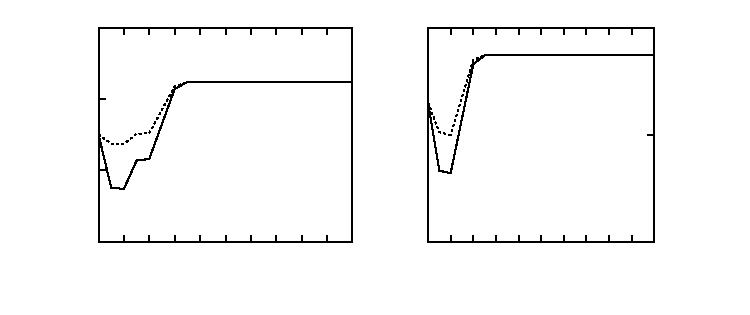
\includegraphics{CL4}}%
    \gplfronttext
  \end{picture}%
\endgroup
}
\resizebox{\textwidth}{!}{% GNUPLOT: LaTeX picture with Postscript
\begingroup
  \makeatletter
  \providecommand\color[2][]{%
    \GenericError{(gnuplot) \space\space\space\@spaces}{%
      Package color not loaded in conjunction with
      terminal option `colourtext'%
    }{See the gnuplot documentation for explanation.%
    }{Either use 'blacktext' in gnuplot or load the package
      color.sty in LaTeX.}%
    \renewcommand\color[2][]{}%
  }%
  \providecommand\includegraphics[2][]{%
    \GenericError{(gnuplot) \space\space\space\@spaces}{%
      Package graphicx or graphics not loaded%
    }{See the gnuplot documentation for explanation.%
    }{The gnuplot epslatex terminal needs graphicx.sty or graphics.sty.}%
    \renewcommand\includegraphics[2][]{}%
  }%
  \providecommand\rotatebox[2]{#2}%
  \@ifundefined{ifGPcolor}{%
    \newif\ifGPcolor
    \GPcolorfalse
  }{}%
  \@ifundefined{ifGPblacktext}{%
    \newif\ifGPblacktext
    \GPblacktexttrue
  }{}%
  % define a \g@addto@macro without @ in the name:
  \let\gplgaddtomacro\g@addto@macro
  % define empty templates for all commands taking text:
  \gdef\gplbacktext{}%
  \gdef\gplfronttext{}%
  \makeatother
  \ifGPblacktext
    % no textcolor at all
    \def\colorrgb#1{}%
    \def\colorgray#1{}%
  \else
    % gray or color?
    \ifGPcolor
      \def\colorrgb#1{\color[rgb]{#1}}%
      \def\colorgray#1{\color[gray]{#1}}%
      \expandafter\def\csname LTw\endcsname{\color{white}}%
      \expandafter\def\csname LTb\endcsname{\color{black}}%
      \expandafter\def\csname LTa\endcsname{\color{black}}%
      \expandafter\def\csname LT0\endcsname{\color[rgb]{1,0,0}}%
      \expandafter\def\csname LT1\endcsname{\color[rgb]{0,1,0}}%
      \expandafter\def\csname LT2\endcsname{\color[rgb]{0,0,1}}%
      \expandafter\def\csname LT3\endcsname{\color[rgb]{1,0,1}}%
      \expandafter\def\csname LT4\endcsname{\color[rgb]{0,1,1}}%
      \expandafter\def\csname LT5\endcsname{\color[rgb]{1,1,0}}%
      \expandafter\def\csname LT6\endcsname{\color[rgb]{0,0,0}}%
      \expandafter\def\csname LT7\endcsname{\color[rgb]{1,0.3,0}}%
      \expandafter\def\csname LT8\endcsname{\color[rgb]{0.5,0.5,0.5}}%
    \else
      % gray
      \def\colorrgb#1{\color{black}}%
      \def\colorgray#1{\color[gray]{#1}}%
      \expandafter\def\csname LTw\endcsname{\color{white}}%
      \expandafter\def\csname LTb\endcsname{\color{black}}%
      \expandafter\def\csname LTa\endcsname{\color{black}}%
      \expandafter\def\csname LT0\endcsname{\color{black}}%
      \expandafter\def\csname LT1\endcsname{\color{black}}%
      \expandafter\def\csname LT2\endcsname{\color{black}}%
      \expandafter\def\csname LT3\endcsname{\color{black}}%
      \expandafter\def\csname LT4\endcsname{\color{black}}%
      \expandafter\def\csname LT5\endcsname{\color{black}}%
      \expandafter\def\csname LT6\endcsname{\color{black}}%
      \expandafter\def\csname LT7\endcsname{\color{black}}%
      \expandafter\def\csname LT8\endcsname{\color{black}}%
    \fi
  \fi
  \setlength{\unitlength}{0.0500bp}%
  \begin{picture}(7200.00,3024.00)%
    \gplgaddtomacro\gplbacktext{%
      \csname LTb\endcsname%
      \put(814,704){\makebox(0,0)[r]{\strut{} 0}}%
      \put(814,1732){\makebox(0,0)[r]{\strut{} 10}}%
      \put(814,2759){\makebox(0,0)[r]{\strut{} 20}}%
      \put(946,484){\makebox(0,0){\strut{} 0}}%
      \put(1190,484){\makebox(0,0){\strut{} 2}}%
      \put(1433,484){\makebox(0,0){\strut{} 4}}%
      \put(1677,484){\makebox(0,0){\strut{} 6}}%
      \put(1921,484){\makebox(0,0){\strut{} 8}}%
      \put(2165,484){\makebox(0,0){\strut{} 10}}%
      \put(2408,484){\makebox(0,0){\strut{} 12}}%
      \put(2652,484){\makebox(0,0){\strut{} 14}}%
      \put(2896,484){\makebox(0,0){\strut{} 16}}%
      \put(3139,484){\makebox(0,0){\strut{} 18}}%
      \put(3383,484){\makebox(0,0){\strut{} 20}}%
      \put(176,1731){\rotatebox{-270}{\makebox(0,0){\strut{}Inventory}}}%
      \put(2164,154){\makebox(0,0){\strut{}Time}}%
      \put(1921,2245){\makebox(0,0)[l]{\strut{}$\omega = 0.8$}}%
    }%
    \gplgaddtomacro\gplfronttext{%
    }%
    \gplgaddtomacro\gplbacktext{%
      \csname LTb\endcsname%
      \put(4109,484){\makebox(0,0){\strut{} 0}}%
      \put(4326,484){\makebox(0,0){\strut{} 2}}%
      \put(4544,484){\makebox(0,0){\strut{} 4}}%
      \put(4761,484){\makebox(0,0){\strut{} 6}}%
      \put(4978,484){\makebox(0,0){\strut{} 8}}%
      \put(5196,484){\makebox(0,0){\strut{} 10}}%
      \put(5413,484){\makebox(0,0){\strut{} 12}}%
      \put(5630,484){\makebox(0,0){\strut{} 14}}%
      \put(5847,484){\makebox(0,0){\strut{} 16}}%
      \put(6065,484){\makebox(0,0){\strut{} 18}}%
      \put(6282,484){\makebox(0,0){\strut{} 20}}%
      \put(6414,704){\makebox(0,0)[l]{\strut{} 0}}%
      \put(6414,1389){\makebox(0,0)[l]{\strut{} 10}}%
      \put(6414,2074){\makebox(0,0)[l]{\strut{} 20}}%
      \put(6414,2759){\makebox(0,0)[l]{\strut{} 30}}%
      \put(7051,1731){\rotatebox{-270}{\makebox(0,0){\strut{}Inventory}}}%
      \put(5195,154){\makebox(0,0){\strut{}Time}}%
    }%
    \gplgaddtomacro\gplfronttext{%
    }%
    \gplbacktext
    \put(0,0){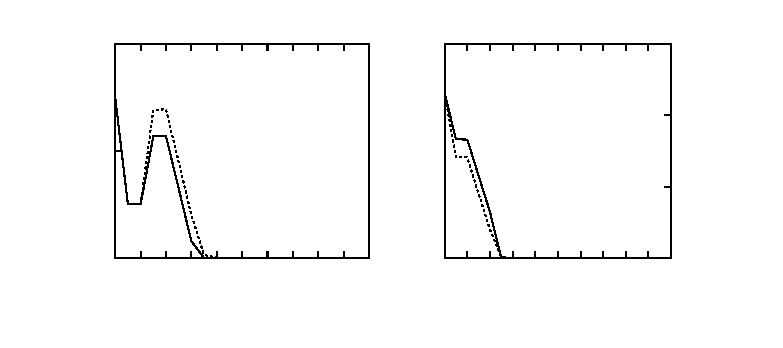
\includegraphics{CL8}}%
    \gplfronttext
  \end{picture}%
\endgroup
}
\caption{Closed-loop response for $\omega = 0.2$ (top), $\omega = 0.4$
(middle) and $\omega = 0.8$ (bottom)}
\label{fig:CL}
\end{figure*}

In Table \ref{tab:CL}, we compare the economic cost incurred in using
the three controllers: (i) Multiobjective MPC $\ell(x,u;z_p)$, (ii)
Economic MPC $\ell_E(x,u)$ and (iii) Tracking MPC to the steady-state
of the multiobjective MPC $\ell_T(x,u,z_s)$. 

\begin{table*}
\caption{Economic cost of implementing MPC}
\label{tab:CL}
\begin{center}
\begin{tabular}{cccc}\toprule
$\omega$ & Multiobjective$ _{ \times 10^{4}}$ & Tracking$ _{ \times 10^{4}}$ & Economic$ _{ \times 10^{4}}$ \\
%& \hfill$ _{ \times 10^{4}}$ & \hfill$_{\times 10^{4}}$ &\hfill
%$_{\times 10^{4}}$ \\
\midrule
0 & 4.4342 & 4.4342 & infeasible \\
0.2 & 4.0246 & 4.0645 & infeasible \\
0.4 & 3.5617 & 3.6252 & infeasible \\
0.6 & 2.7343 & 2.7380 & 2.7380 (stabilizes origin) \\
0.8 & 2.2670 & 2.2670 & 2.2670 \\
1.0 & 2.2670 & 2.2670 & 2.2670 \\
\bottomrule
\end{tabular}
\end{center}
\end{table*}
{\em{todo: run simulation for w=0.6 again}}

We observe that as $\omega$ increases, that is, as the economic costs
are given more weighting, the steady-state approaches the constraint
boundary. In such situations, the optimal input profile is dominated
by feasibility and as such all the three stage costs incur the same
economic cost in the closed loop. However, for intermediate values of
$\omega$, that is, when the practitioner has comparable weighting to
both tracking the safety stock and minimizing costs,
multiobjective-MPC gives the best performance. While in the tracking
MPC, we can design the system go to the same steady-state as multiobjective, the absence of
economic knowledge in the tracking stage cost means that some
economically more attractive transients are not considered by the
online optimizer. While designing a controller that minimizes only the
costs seems very attractive, the drawback is that for supply chains, such economic MPC can only stabilize steady states
that lie on the one of the vertices of the constraint set. Therefore,
we cannot use pure economic MPC to track the inventories to a target
value (we can design the economic MPC to stabilize a target
value). Also, since we can guarantee stability for pure economic MPC
only with the terminal equality constraint, its region of attraction (the
region of the state-space where the MPC controller is defined) is much
smaller than the multiobjective controller, which has a much larger
terminal region $\mathbb{X}_f$. 

\section{Multi-product, multi-echelon supply chain example}
\label{sec:multi_example}
In this section, we follow the design procedure described in the
previous section to implement model predictive control for a
multi-product, multi-echelon supply chain. The supply chain that is
studied is shown in Figure \ref{fig:lssc}. It consists of a
manufacturing facility $M1$ that supplies two products $A,B$ to two
distribution centers $D1,D2$ and a retailer $R5$. Distribution center
$D1$ supplies the products to retailers $R1,R2$ while distribution
center $D2$ supplies to $R3$ and $R4$. 

\begin{figure*}
\centering
\scriptsize
\resizebox{0.5\textwidth}{!}{\begin{picture}(0,0)%
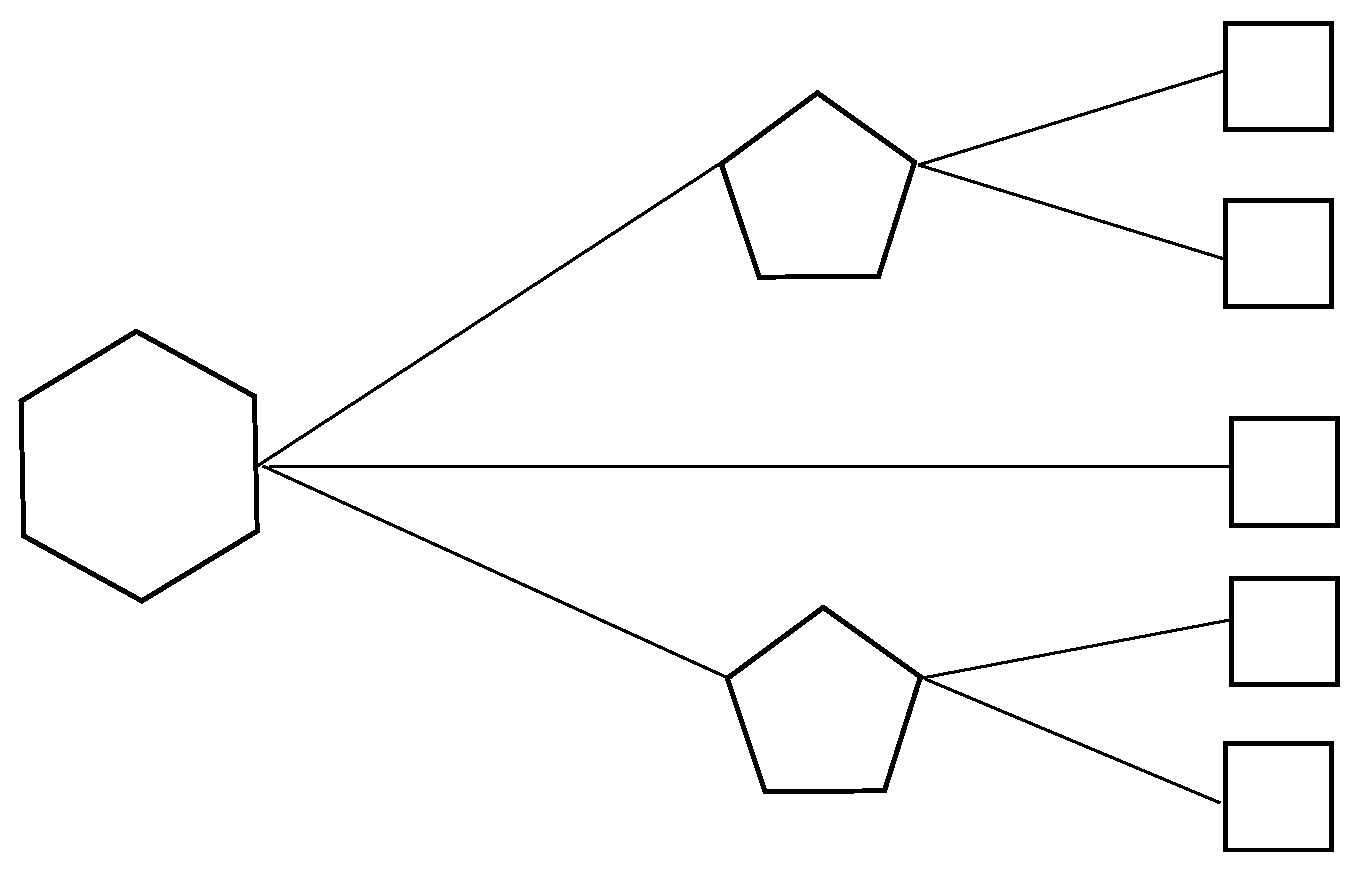
\includegraphics{esc/lssc}%
\end{picture}%
\setlength{\unitlength}{4144sp}%
%
\begingroup\makeatletter\ifx\SetFigFont\undefined%
\gdef\SetFigFont#1#2#3#4#5{%
  \reset@font\fontsize{#1}{#2pt}%
  \fontfamily{#3}\fontseries{#4}\fontshape{#5}%
  \selectfont}%
\fi\endgroup%
\begin{picture}(10101,6366)(1363,-5719)
\put(10801,164){\makebox(0,0)[lb]{\smash{{\SetFigFont{17}{20.4}{\familydefault}{\mddefault}{\updefault}{\color[rgb]{0,0,0}$R1$}%
}}}}
\put(2071,-2851){\makebox(0,0)[lb]{\smash{{\SetFigFont{17}{20.4}{\familydefault}{\mddefault}{\updefault}{\color[rgb]{0,0,0}$M1$}%
}}}}
\put(7246,-736){\makebox(0,0)[lb]{\smash{{\SetFigFont{17}{20.4}{\familydefault}{\mddefault}{\updefault}{\color[rgb]{0,0,0}$D1$}%
}}}}
\put(7291,-4741){\makebox(0,0)[lb]{\smash{{\SetFigFont{17}{20.4}{\familydefault}{\mddefault}{\updefault}{\color[rgb]{0,0,0}$D2$}%
}}}}
\put(10801,-5371){\makebox(0,0)[lb]{\smash{{\SetFigFont{17}{20.4}{\familydefault}{\mddefault}{\updefault}{\color[rgb]{0,0,0}$R4$}%
}}}}
\put(10846,-4111){\makebox(0,0)[lb]{\smash{{\SetFigFont{17}{20.4}{\familydefault}{\mddefault}{\updefault}{\color[rgb]{0,0,0}$R3$}%
}}}}
\put(10891,-2896){\makebox(0,0)[lb]{\smash{{\SetFigFont{17}{20.4}{\familydefault}{\mddefault}{\updefault}{\color[rgb]{0,0,0}$R5$}%
}}}}
\put(10801,-1231){\makebox(0,0)[lb]{\smash{{\SetFigFont{17}{20.4}{\familydefault}{\mddefault}{\updefault}{\color[rgb]{0,0,0}$R2$}%
}}}}
\end{picture}%
}
\caption{Multi-product, Multi-echelon supply chain studied}
\label{fig:lssc}
\end{figure*}

We list the production lead-times at the manufacturing facility in
Table \ref{tab:prodlead}. We assume that the manufacturing facility is
able to produce both products simultaneously, with the only limitation
being the combined storage of these products in the manufacturing
node's storage facility (see Table \ref{tab:constraints}).
 
\begin{table*}
\caption{Production lead-times}
\label{tab:prodlead}
\begin{center}
\begin{tabular}{cc}\toprule
Product& Lead-time \\
\midrule
$A$ & 2\\
$B$ & 3\\
\bottomrule
\end{tabular}
\end{center}
\end{table*}

In Table \ref{tab:translead}, we list the transportation times between
each node. 
\begin{table*}
\caption{Transportation lead-times}
\label{tab:translead}
\begin{center}
\begin{tabular}{cccccccc}\toprule
& $D1$ & $D2$  & $R1$ & $R2$ & $R3$ & $R4$ & $R5$ \\
\midrule
$M1$ &2&1& & & & &4\\
$D1$ & & &1&1& & & \\
$D2$ & & & & &2&1& \\
\bottomrule
\end{tabular}
\end{center}
\end{table*}


The retailers respond to customer demands which is assumed to arrive
at each period following a normal distribution around a nominal
demand. The nominal demand for each retailer node is listed in Table
\ref{tab:nomdem} while the variance of the demand signal in each retailer node for
both products are listed in Table \ref{tab:vardem}

\begin{table*}
\caption{Nominal demand}
\begin{center}
\begin{tabular}{cccccc}\toprule
\label{tab:nomdem}
 &$R1$&$R2$&$R3$&$R4$&$R5$\\
\midrule
$A$&3.0&4.5&5.0&2.0&4.0\\
$B$&4.2&3.1&1.4&2.5&4.2\\
\bottomrule
\end{tabular}
\end{center}
\end{table*}

\begin{table*}
\caption{Variance of  demand}
\begin{center}
\begin{tabular}{cccccc}\toprule
\label{tab:vardem}
 &$R1$&$R2$&$R3$&$R4$&$R5$\\
\midrule
$A$&1.1&1.3&1.1&1.2&1.4\\
$B$&1.3&1.4&1.1&1.1&1.4\\
\bottomrule
\end{tabular}
\end{center}
\end{table*}

For each node, we choose the target inventory to be the amount of
product to be carried so that demands can be met for as long as the
longest delay in the supply chain. The longest delay in the supply
chain is 4 (the transportation time between $M1$ and $R5$). Hence, for
the retailers, we choose the target inventory to be four time the
nominal demand. For the distributors, the target inventory is four
times the nominal demand at the distributor. The nominal demand at the
distributor is the sum of the demands at the retailers that is served
by the distributor. 

\begin{table*}
\caption{Target inventories}
\label{tab:targinv}
\begin{center}
\begin{tabular}{ccccccccc}\toprule
& $M1$ & $D1$ & $D2$  & $R1$ & $R2$ & $R3$ & $R4$ & $R5$ \\
\midrule
$A$&70&30  &24   &12  &18  &20 &8 &16\\
$B$&61&29.2&15.6 &16.8&12.4&5.6&10&16.8 \\
\bottomrule
\end{tabular}
\end{center}
\end{table*}

The target back-orders in each node is $0$.

As mentioned earlier, each node has a combined inventory storage
capacity. This capacity is listed in Table \ref{tab:constraints}. The
maximum storage is chosen to be greater than the target inventories.
\begin{table*}
\caption{Capacity constraints}
\label{tab:constraints}
\begin{center}
\begin{tabular}{ccccccccc}\toprule
& $M1$ & $D1$ & $D2$  & $R1$ & $R2$ & $R3$ & $R4$ & $R5$ \\
\midrule
$\Inv_A+\Inv_B$&140&80  &50   &40  &40  &30 &25 &45\\
\bottomrule
\end{tabular}
\end{center}
\end{table*}

The economic objective is the sum of the (i) inventory holding costs
(ii) back-order costs and (iii) shipping and ordering costs. The
coefficients for these costs are listed in the following tables.

\begin{table*}
\caption{State economic costs}
\label{tab:state_economic}
\begin{center}
\begin{tabular}{ccccccccc}\toprule
& $M1$ & $D1$ & $D2$  & $R1$ & $R2$ & $R3$ & $R4$ & $R5$ \\
\midrule
Inventory holding&1&1  &1   &1  &1  &1 &1 &1\\
Back-order&10&10&10 &10&10&10&10&10 \\
\bottomrule
\end{tabular}
\end{center}
\end{table*}

\begin{table*}
\caption{Input costs}
\label{tab:input_economic}
\begin{center}
\begin{tabular}{cccccccc}\toprule
& $D1$ & $D2$  & $R1$ & $R2$ & $R3$ & $R4$ & $R5$ \\
\midrule
$M1$ &(4,2)&(1,2)& & & & &(5,4)\\
$D1$ & & &(1,1)&(1,1)& & & \\
$D2$ & & & & &(2,2)&(1.5,1.5)& \\
\bottomrule
\end{tabular}
\end{center}
\end{table*}

In table \ref{tab:input_economic}, each entry corresponds to the
shipping cost of product $A$ and product $B$ respectively. In
addition, the cost coefficient of shipping products to the
customers from the retailers is $1$.

The ordering costs coefficients are all chosen to be $1$, except for
ordering between the $R5$ and $M1$ in which the cost-coefficient is
chosen to be $0.5$. 

The production costs for product $A$ is 10 per unit while that for $B$
is 4 per unit.


The tracking objective is a weighted sum of the squares of the
deviation of the inventories(and backorders) from their targets. These
weights are chosen as $1$ for inventory deviation (that is, we
penalize $(\Inv-\Inv_t)^2$, 10 for backorder deviation
($10(\BO-\BO_t)^2$). The inputs are penalized from their targets with
a weight of $0.1$ (the input targets are chosen to be the steady-state
values as described below).


With the aforementioned details about the supply chain, the supply
chain model can be written in the state-space format \eqref{eq:model} and the stage
costs $\ell_E(\cdot,\cdot)$, \eqref{eq:ellE} and
$\ell_T(\cdot,\cdot)$, \eqref{eq:ellT} is defined.  Choosing an
economic objective weight of $0.4$, we can solve for the steady-state
problem \eqref{eq:SSMulti} to obtain the steady state. As discussed in
the previous section, the multiobjective steady state lies between a
pure tracking ($\omega = 0$) and a pure economic $(\omega=1)$ steady
state. We re-iterate that the input steady-state remains the same
irrespective of the objective function, because of the steady-state
constraint that fixes all the flows in the supply chain in accordance
with the nominal demand. In Table \ref{tab:steady}, we list the
inventory steady-states (for product-A) for the pure economic, tracking and the
multiobjective cost functions.


\begin{table*}
\caption{Steady state  inventories for product $A$}
\label{tab:steady}
\begin{center}
\begin{tabular}{ccccccccc}\toprule
& $M1$ & $D1$ & $D2$  & $R1$ & $R2$ & $R3$ & $R4$ & $R5$ \\
\midrule
Tracking                      &70   &30   &24   &12&18  &20  &8&16 \\
Economic                      &0    &0    &0    &0 &0   &0   &0&0   \\
Multiobjective($\omega = 0.4$)&57.93&17.93&11.93&0 &5.93&7.93&0&3.93\\
\bottomrule
\end{tabular}
\end{center}
\end{table*}

\paragraph{$(\sigma,\Sigma) $ Policy.} We compare the closed-loop operation of
the centralized multi-objective supply chain with that of the
closed-loop dynamics due to a $(\sigma,\Sigma) $ policy. In the $(\sigma,\Sigma) $
policy, the nodes orders according to the
following shipping and ordering policies.. We denote the shipments coming from the upstream
node as $S^{u}$, while the orders coming from downstream (demand for
the retailer as $O^{d}$.
\begin{equation}
S(t) = \begin{cases} O^{d}(t)+\BO(t) \\\quad \text{if~}
  \Inv(t)+S^{u}(t)-(O^{d}(t)+\BO(t)) \geq 0 \\
  \Inv(t)+S^{u}(t)\quad \text{otherwise}
  \end{cases}
\end{equation}

Having determined the shipment at time $k$, the node then places
orders according to the inventory and backorder levels that the
shipments will lead to at the next time as:
\begin{equation}
O(t) = \begin{cases} \Sigma - (\Inv(t+1)-\BO(t+1))\\ \quad
  \text{if~} (\Inv(t+1)-\BO(t+1)) \leq \sigma\\
0 \quad \text{otherwise~}
\end{cases}
\end{equation}

The $(\sigma,\Sigma)$ policy is a decentralized linear feedback policy. The retailer
observes the demands, makes its ordering decisions which is then used
by the distributor and so on. 

\subsection{Results}
The supply chain described in the previous section was simulated for
50 days using a stochastic demand signal. The terminal
condition used was that the system should be at the steady-state
(\ref{subsec:terminal_equality}) at the end of the prediction horizon,
which was chosen as 15 days. Furthermore, we assumed that the MPC
controller had perfect demand information for three days. For the
remainder of the prediction horizon, we used the nominal demands as
the demand forecast. For the $(\sigma,\Sigma)$ policy, we chose
$\sigma = 0.7\Sigma$ and $\Sigma$ as the steady state inventory. 

The initial inventories of the nodes were chosen as follows:
\begin{table*}
\caption{Initial inventories}
\label{tab:initial}
\begin{center}
\begin{tabular}{ccccccccc}\toprule
& $M1$ & $D1$ & $D2$  & $R1$ & $R2$ & $R3$ & $R4$ & $R5$ \\
\midrule
$A$                      &63   &14   &24   &0 &2.1  &3.1  &3.1&0 \\
$B$                      &40   &12   &7    &0 &1.2  &1.2  &0  &5.2   \\
\bottomrule
\end{tabular}
\end{center}
\end{table*}
All the backorders were $0$ and the inputs were at their steady-state
at the begining of the simulation.

In Figure \ref{fig:bullwhip}, we report the ordering-profile in the supply
chain, and compare the variance of the demands observed with the
variance of the orders placed as we move upstream in the node. The
variance in orders placed as we move upstream is an measure of the
bullwhip effect. We see that the the MPC policy has less variance in
ordering profile as we move upstream in the supply chain. This is
because the MPC controller is a centralized controller that not only
considers all the nodes together, but also makes predictions for two
weeks into the future. Therefore, at certain nodes, it is able to take
advantage of higher inventory levels than the steady-state inventory
to place fewer orders in total. The $(\sigma,\Sigma)$ policy shows the
classical bullwhip effect of the variance of the orders increasing as
we move upstream. 

\begin{figure*}
\centering
\scriptsize
\resizebox{0.5\textwidth}{!}{% GNUPLOT: LaTeX picture with Postscript
\begingroup
  \makeatletter
  \providecommand\color[2][]{%
    \GenericError{(gnuplot) \space\space\space\@spaces}{%
      Package color not loaded in conjunction with
      terminal option `colourtext'%
    }{See the gnuplot documentation for explanation.%
    }{Either use 'blacktext' in gnuplot or load the package
      color.sty in LaTeX.}%
    \renewcommand\color[2][]{}%
  }%
  \providecommand\includegraphics[2][]{%
    \GenericError{(gnuplot) \space\space\space\@spaces}{%
      Package graphicx or graphics not loaded%
    }{See the gnuplot documentation for explanation.%
    }{The gnuplot epslatex terminal needs graphicx.sty or graphics.sty.}%
    \renewcommand\includegraphics[2][]{}%
  }%
  \providecommand\rotatebox[2]{#2}%
  \@ifundefined{ifGPcolor}{%
    \newif\ifGPcolor
    \GPcolortrue
  }{}%
  \@ifundefined{ifGPblacktext}{%
    \newif\ifGPblacktext
    \GPblacktexttrue
  }{}%
  % define a \g@addto@macro without @ in the name:
  \let\gplgaddtomacro\g@addto@macro
  % define empty templates for all commands taking text:
  \gdef\gplbacktext{}%
  \gdef\gplfronttext{}%
  \makeatother
  \ifGPblacktext
    % no textcolor at all
    \def\colorrgb#1{}%
    \def\colorgray#1{}%
  \else
    % gray or color?
    \ifGPcolor
      \def\colorrgb#1{\color[rgb]{#1}}%
      \def\colorgray#1{\color[gray]{#1}}%
      \expandafter\def\csname LTw\endcsname{\color{white}}%
      \expandafter\def\csname LTb\endcsname{\color{black}}%
      \expandafter\def\csname LTa\endcsname{\color{black}}%
      \expandafter\def\csname LT0\endcsname{\color[rgb]{1,0,0}}%
      \expandafter\def\csname LT1\endcsname{\color[rgb]{0,1,0}}%
      \expandafter\def\csname LT2\endcsname{\color[rgb]{0,0,1}}%
      \expandafter\def\csname LT3\endcsname{\color[rgb]{1,0,1}}%
      \expandafter\def\csname LT4\endcsname{\color[rgb]{0,1,1}}%
      \expandafter\def\csname LT5\endcsname{\color[rgb]{1,1,0}}%
      \expandafter\def\csname LT6\endcsname{\color[rgb]{0,0,0}}%
      \expandafter\def\csname LT7\endcsname{\color[rgb]{1,0.3,0}}%
      \expandafter\def\csname LT8\endcsname{\color[rgb]{0.5,0.5,0.5}}%
    \else
      % gray
      \def\colorrgb#1{\color{black}}%
      \def\colorgray#1{\color[gray]{#1}}%
      \expandafter\def\csname LTw\endcsname{\color{white}}%
      \expandafter\def\csname LTb\endcsname{\color{black}}%
      \expandafter\def\csname LTa\endcsname{\color{black}}%
      \expandafter\def\csname LT0\endcsname{\color{black}}%
      \expandafter\def\csname LT1\endcsname{\color{black}}%
      \expandafter\def\csname LT2\endcsname{\color{black}}%
      \expandafter\def\csname LT3\endcsname{\color{black}}%
      \expandafter\def\csname LT4\endcsname{\color{black}}%
      \expandafter\def\csname LT5\endcsname{\color{black}}%
      \expandafter\def\csname LT6\endcsname{\color{black}}%
      \expandafter\def\csname LT7\endcsname{\color{black}}%
      \expandafter\def\csname LT8\endcsname{\color{black}}%
    \fi
  \fi
  \setlength{\unitlength}{0.0500bp}%
  \begin{picture}(7200.00,3024.00)%
    \gplgaddtomacro\gplbacktext{%
      \csname LTb\endcsname%
      \put(682,846){\makebox(0,0)[r]{\strut{} 0}}%
      \put(682,1119){\makebox(0,0)[r]{\strut{} 1}}%
      \put(682,1393){\makebox(0,0)[r]{\strut{} 2}}%
      \put(682,1666){\makebox(0,0)[r]{\strut{} 3}}%
      \put(682,1939){\makebox(0,0)[r]{\strut{} 4}}%
      \put(682,2212){\makebox(0,0)[r]{\strut{} 5}}%
      \put(682,2486){\makebox(0,0)[r]{\strut{} 6}}%
      \put(682,2759){\makebox(0,0)[r]{\strut{} 7}}%
      \put(2012,714){\rotatebox{-45}{\makebox(0,0)[l]{\strut{}R1}}}%
      \put(3210,714){\rotatebox{-45}{\makebox(0,0)[l]{\strut{}R5}}}%
      \put(4407,714){\rotatebox{-45}{\makebox(0,0)[l]{\strut{}D1}}}%
      \put(5605,714){\rotatebox{-45}{\makebox(0,0)[l]{\strut{}D2}}}%
      \put(176,1802){\rotatebox{-270}{\makebox(0,0){\strut{}Standard deviation of Orders}}}%
    }%
    \gplgaddtomacro\gplfronttext{%
      \csname LTb\endcsname%
      \put(1998,173){\makebox(0,0)[r]{\strut{}Incoming}}%
      \csname LTb\endcsname%
      \put(3909,173){\makebox(0,0)[r]{\strut{}MPC}}%
      \csname LTb\endcsname%
      \put(5820,173){\makebox(0,0)[r]{\strut{}$(\sigma,\Sigma)$}}%
    }%
    \gplbacktext
    \put(0,0){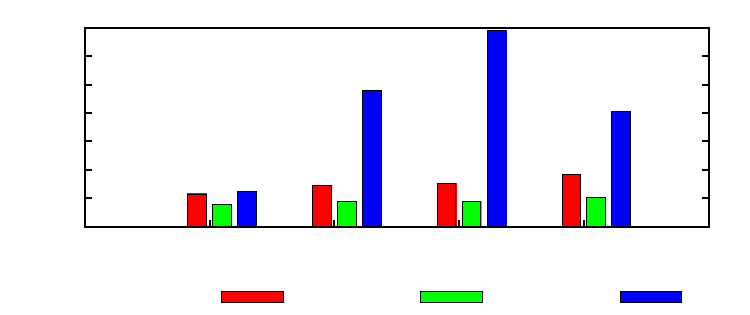
\includegraphics{esc/bullwhip}}%
    \gplfronttext
  \end{picture}%
\endgroup
}
\caption{Bullwhip effect}
\label{fig:bullwhip}
\end{figure*}

In Figure \ref{fig:Order}, we plot the orders placed by the MPC
controller and the $(\sigma,\Sigma)$ policy controller in response to
demands of product $A$ at Retailer $R3$.

\begin{figure*}
\centering
\scriptsize
\resizebox{0.5\textwidth}{!}{% GNUPLOT: LaTeX picture with Postscript
\begingroup
  \makeatletter
  \providecommand\color[2][]{%
    \GenericError{(gnuplot) \space\space\space\@spaces}{%
      Package color not loaded in conjunction with
      terminal option `colourtext'%
    }{See the gnuplot documentation for explanation.%
    }{Either use 'blacktext' in gnuplot or load the package
      color.sty in LaTeX.}%
    \renewcommand\color[2][]{}%
  }%
  \providecommand\includegraphics[2][]{%
    \GenericError{(gnuplot) \space\space\space\@spaces}{%
      Package graphicx or graphics not loaded%
    }{See the gnuplot documentation for explanation.%
    }{The gnuplot epslatex terminal needs graphicx.sty or graphics.sty.}%
    \renewcommand\includegraphics[2][]{}%
  }%
  \providecommand\rotatebox[2]{#2}%
  \@ifundefined{ifGPcolor}{%
    \newif\ifGPcolor
    \GPcolortrue
  }{}%
  \@ifundefined{ifGPblacktext}{%
    \newif\ifGPblacktext
    \GPblacktexttrue
  }{}%
  % define a \g@addto@macro without @ in the name:
  \let\gplgaddtomacro\g@addto@macro
  % define empty templates for all commands taking text:
  \gdef\gplbacktext{}%
  \gdef\gplfronttext{}%
  \makeatother
  \ifGPblacktext
    % no textcolor at all
    \def\colorrgb#1{}%
    \def\colorgray#1{}%
  \else
    % gray or color?
    \ifGPcolor
      \def\colorrgb#1{\color[rgb]{#1}}%
      \def\colorgray#1{\color[gray]{#1}}%
      \expandafter\def\csname LTw\endcsname{\color{white}}%
      \expandafter\def\csname LTb\endcsname{\color{black}}%
      \expandafter\def\csname LTa\endcsname{\color{black}}%
      \expandafter\def\csname LT0\endcsname{\color[rgb]{1,0,0}}%
      \expandafter\def\csname LT1\endcsname{\color[rgb]{0,1,0}}%
      \expandafter\def\csname LT2\endcsname{\color[rgb]{0,0,1}}%
      \expandafter\def\csname LT3\endcsname{\color[rgb]{1,0,1}}%
      \expandafter\def\csname LT4\endcsname{\color[rgb]{0,1,1}}%
      \expandafter\def\csname LT5\endcsname{\color[rgb]{1,1,0}}%
      \expandafter\def\csname LT6\endcsname{\color[rgb]{0,0,0}}%
      \expandafter\def\csname LT7\endcsname{\color[rgb]{1,0.3,0}}%
      \expandafter\def\csname LT8\endcsname{\color[rgb]{0.5,0.5,0.5}}%
    \else
      % gray
      \def\colorrgb#1{\color{black}}%
      \def\colorgray#1{\color[gray]{#1}}%
      \expandafter\def\csname LTw\endcsname{\color{white}}%
      \expandafter\def\csname LTb\endcsname{\color{black}}%
      \expandafter\def\csname LTa\endcsname{\color{black}}%
      \expandafter\def\csname LT0\endcsname{\color{black}}%
      \expandafter\def\csname LT1\endcsname{\color{black}}%
      \expandafter\def\csname LT2\endcsname{\color{black}}%
      \expandafter\def\csname LT3\endcsname{\color{black}}%
      \expandafter\def\csname LT4\endcsname{\color{black}}%
      \expandafter\def\csname LT5\endcsname{\color{black}}%
      \expandafter\def\csname LT6\endcsname{\color{black}}%
      \expandafter\def\csname LT7\endcsname{\color{black}}%
      \expandafter\def\csname LT8\endcsname{\color{black}}%
    \fi
  \fi
  \setlength{\unitlength}{0.0500bp}%
  \begin{picture}(7200.00,3024.00)%
    \gplgaddtomacro\gplbacktext{%
      \csname LTb\endcsname%
      \put(594,704){\makebox(0,0)[r]{\strut{} 0}}%
      \put(594,1732){\makebox(0,0)[r]{\strut{} 10}}%
      \put(594,2759){\makebox(0,0)[r]{\strut{} 20}}%
      \put(726,484){\makebox(0,0){\strut{} 0}}%
      \put(1941,484){\makebox(0,0){\strut{} 10}}%
      \put(3157,484){\makebox(0,0){\strut{} 20}}%
      \put(4372,484){\makebox(0,0){\strut{} 30}}%
      \put(5588,484){\makebox(0,0){\strut{} 40}}%
      \put(6803,484){\makebox(0,0){\strut{} 50}}%
      \put(3764,154){\makebox(0,0){\strut{}Time}}%
    }%
    \gplgaddtomacro\gplfronttext{%
      \csname LTb\endcsname%
      \put(5816,2586){\makebox(0,0)[r]{\strut{}Customer demand}}%
      \csname LTb\endcsname%
      \put(5816,2366){\makebox(0,0)[r]{\strut{}Orders placed-MPC}}%
      \csname LTb\endcsname%
      \put(5816,2146){\makebox(0,0)[r]{\strut{}Orders placed-$(\sigma,\Sigma)$}}%
    }%
    \gplbacktext
    \put(0,0){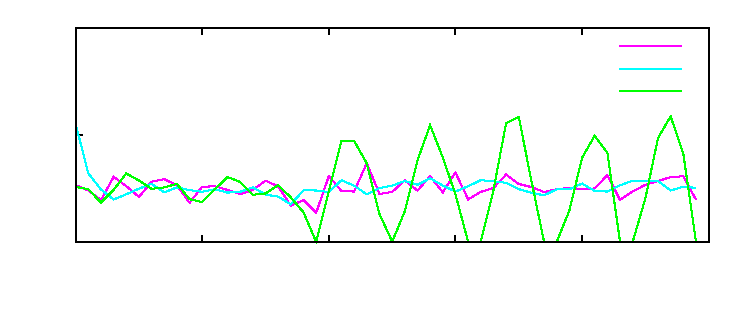
\includegraphics{esc/R5}}%
    \gplfronttext
  \end{picture}%
\endgroup
}
\caption{Ordering profile at $R3$}
\label{fig:Order}
\end{figure*}

In Figure \ref{fig:R3}, we plot the inventory and the
back-order of  of the product $A$
at retailer $R3$. Note that the steady-state for product $A$ was
7.93. 

\begin{figure*}
\centering
\scriptsize
\resizebox{1\textwidth}{!}{% GNUPLOT: LaTeX picture with Postscript
\begingroup
  \makeatletter
  \providecommand\color[2][]{%
    \GenericError{(gnuplot) \space\space\space\@spaces}{%
      Package color not loaded in conjunction with
      terminal option `colourtext'%
    }{See the gnuplot documentation for explanation.%
    }{Either use 'blacktext' in gnuplot or load the package
      color.sty in LaTeX.}%
    \renewcommand\color[2][]{}%
  }%
  \providecommand\includegraphics[2][]{%
    \GenericError{(gnuplot) \space\space\space\@spaces}{%
      Package graphicx or graphics not loaded%
    }{See the gnuplot documentation for explanation.%
    }{The gnuplot epslatex terminal needs graphicx.sty or graphics.sty.}%
    \renewcommand\includegraphics[2][]{}%
  }%
  \providecommand\rotatebox[2]{#2}%
  \@ifundefined{ifGPcolor}{%
    \newif\ifGPcolor
    \GPcolorfalse
  }{}%
  \@ifundefined{ifGPblacktext}{%
    \newif\ifGPblacktext
    \GPblacktexttrue
  }{}%
  % define a \g@addto@macro without @ in the name:
  \let\gplgaddtomacro\g@addto@macro
  % define empty templates for all commands taking text:
  \gdef\gplbacktext{}%
  \gdef\gplfronttext{}%
  \makeatother
  \ifGPblacktext
    % no textcolor at all
    \def\colorrgb#1{}%
    \def\colorgray#1{}%
  \else
    % gray or color?
    \ifGPcolor
      \def\colorrgb#1{\color[rgb]{#1}}%
      \def\colorgray#1{\color[gray]{#1}}%
      \expandafter\def\csname LTw\endcsname{\color{white}}%
      \expandafter\def\csname LTb\endcsname{\color{black}}%
      \expandafter\def\csname LTa\endcsname{\color{black}}%
      \expandafter\def\csname LT0\endcsname{\color[rgb]{1,0,0}}%
      \expandafter\def\csname LT1\endcsname{\color[rgb]{0,1,0}}%
      \expandafter\def\csname LT2\endcsname{\color[rgb]{0,0,1}}%
      \expandafter\def\csname LT3\endcsname{\color[rgb]{1,0,1}}%
      \expandafter\def\csname LT4\endcsname{\color[rgb]{0,1,1}}%
      \expandafter\def\csname LT5\endcsname{\color[rgb]{1,1,0}}%
      \expandafter\def\csname LT6\endcsname{\color[rgb]{0,0,0}}%
      \expandafter\def\csname LT7\endcsname{\color[rgb]{1,0.3,0}}%
      \expandafter\def\csname LT8\endcsname{\color[rgb]{0.5,0.5,0.5}}%
    \else
      % gray
      \def\colorrgb#1{\color{black}}%
      \def\colorgray#1{\color[gray]{#1}}%
      \expandafter\def\csname LTw\endcsname{\color{white}}%
      \expandafter\def\csname LTb\endcsname{\color{black}}%
      \expandafter\def\csname LTa\endcsname{\color{black}}%
      \expandafter\def\csname LT0\endcsname{\color{black}}%
      \expandafter\def\csname LT1\endcsname{\color{black}}%
      \expandafter\def\csname LT2\endcsname{\color{black}}%
      \expandafter\def\csname LT3\endcsname{\color{black}}%
      \expandafter\def\csname LT4\endcsname{\color{black}}%
      \expandafter\def\csname LT5\endcsname{\color{black}}%
      \expandafter\def\csname LT6\endcsname{\color{black}}%
      \expandafter\def\csname LT7\endcsname{\color{black}}%
      \expandafter\def\csname LT8\endcsname{\color{black}}%
    \fi
  \fi
  \setlength{\unitlength}{0.0500bp}%
  \begin{picture}(7200.00,3024.00)%
    \gplgaddtomacro\gplbacktext{%
      \csname LTb\endcsname%
      \put(594,946){\makebox(0,0)[r]{\strut{} 0}}%
      \put(594,2155){\makebox(0,0)[r]{\strut{} 10}}%
      \put(828,484){\makebox(0,0){\strut{} 0}}%
      \put(1339,484){\makebox(0,0){\strut{} 10}}%
      \put(1850,484){\makebox(0,0){\strut{} 20}}%
      \put(2361,484){\makebox(0,0){\strut{} 30}}%
      \put(2872,484){\makebox(0,0){\strut{} 40}}%
      \put(3383,484){\makebox(0,0){\strut{} 50}}%
      \put(2054,154){\makebox(0,0){\strut{}Time}}%
    }%
    \gplgaddtomacro\gplfronttext{%
      \csname LTb\endcsname%
      \put(2396,2586){\makebox(0,0)[r]{\strut{}Inventory}}%
      \csname LTb\endcsname%
      \put(2396,2366){\makebox(0,0)[r]{\strut{}Backorder}}%
    }%
    \gplgaddtomacro\gplbacktext{%
      \csname LTb\endcsname%
      \put(4201,484){\makebox(0,0){\strut{} 0}}%
      \put(4661,484){\makebox(0,0){\strut{} 10}}%
      \put(5121,484){\makebox(0,0){\strut{} 20}}%
      \put(5582,484){\makebox(0,0){\strut{} 30}}%
      \put(6042,484){\makebox(0,0){\strut{} 40}}%
      \put(6502,484){\makebox(0,0){\strut{} 50}}%
      \put(6634,704){\makebox(0,0)[l]{\strut{} 0}}%
      \put(6634,1732){\makebox(0,0)[l]{\strut{} 10}}%
      \put(6634,2759){\makebox(0,0)[l]{\strut{} 20}}%
      \put(5305,154){\makebox(0,0){\strut{}Time}}%
    }%
    \gplgaddtomacro\gplfronttext{%
      \csname LTb\endcsname%
      \put(5779,2586){\makebox(0,0)[r]{\strut{}Customer demand}}%
      \csname LTb\endcsname%
      \put(5779,2366){\makebox(0,0)[r]{\strut{}Orders placed}}%
    }%
    \gplbacktext
    \put(0,0){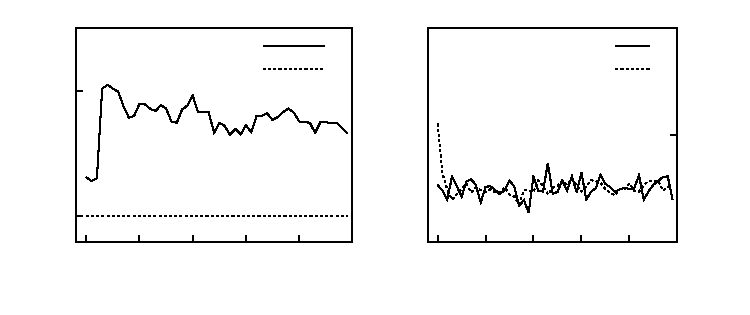
\includegraphics{R3}}%
    \gplfronttext
  \end{picture}%
\endgroup
}
\caption{Inventory and Backorder profile at $R3$}
\label{fig:R3}
\end{figure*}

Finally, in Table \ref{tab:avgA}, we list the
average inventory at each node for products $A$ and $B$. Observe that
the average inventory at the nodes for the MPC policy is much closer
to the steady-state values, indicating that the MPC policy is
stabilizing. This example also illustrates the inherent robustness of
economic MPC as the controller was able to reject small variations in
demand around the nominal demand.

\begin{table*}
\caption{Average inventory for Product-A}
\label{tab:avgA}
\begin{center}
\begin{tabular}{cccccccccc}\toprule
 &$M1$&$D1$&$D2$&$R1$&$R2$&$R3$&$R4$&$R5$\\ \midrule
MPC&58.01&17.48&12.36&0.34&5.43&7.71&0.26&3.44\\ 
Policy&82.91&10.70&6.02&0.011&1.39&3.21&0.23&5.47\\
\bottomrule 
\end{tabular}
\end{center}
\end{table*}
\subsection{Scheduling model}
\label{subsec:scheduling}
In the preceeding sections, we did not consider the scheduling problem
at the manufacturing unit; instead, we approximated the production
delay using a constant production lead-time. In this section, we study
the economic MPC closed-loop performance for a supply chain which
includes a scheduling model for the manufacturing node.

We consider the same supply chain as in the previous section (Fig
\ref{fig:lssc}), but with the following modification. The
manufacturing facility is assumed to have one unit $U$ which can
 make both products $A$ and $B$. The unit needs $3$ time units to make
$A$ via the task $\text{TA}$ and $2$ time units to make $B$ via the task
$\text{TB}$. In addition, there is changeover time of 1 unit whenever the
task is changed from $A$ to $B$ or vice-versa. 

Denote the set $\mathbb{I} = \set{\text{TA},\text{TB}}$,  $\text{PT}(i)$ as the
production lead time for each $i \in \mathbb{I}$ and $\text{CHT}(i,i')$ as
the changeover time between $i$ to $i'$. The scheduling constraints on
the manufacturing node can now be enforced by the following
inequalities:


\begin{alignat}{2}
&\sum_{i\in \mathbb{I}}\sum_{t' = t-\text{PT}(i)+1}^{t}W(i,t')+\sum_{i' \in
 \mathbb{I} \atop i' \neq i}\sum_{t'=t-\text{CHT}(i,i')+1}^{t} Z(i,i',t') \leq 1 & \forall t \nonumber \\
&\sum_{t' = t-PT(i)+1}^{t} W(i,t) \leq Y(i,t) & \forall t, \forall i
\in \mathbb{I} \nonumber\\
&X(i,t) \geq Y(i,t) & \forall t, \forall i \in \mathbb{I} \nonumber\\
&\sum_{i \in \mathbb{I}}X(i,t) = 1 & \forall t  \label{eq:assign}\\
&Z(i,i',t) \leq X(i,t-1) &\forall t, \forall i \in \mathbb{I}, i' \in
\mathbb{I}/i \nonumber\\
&Z(i,i',t) \leq X(i',t) &\forall t, \forall i \in \mathbb{I}, i' \in
\mathbb{I}/i \nonumber \\
&Z(i,i',t) \geq X(i,t-1)+X(i',t)-1 &\forall t, \forall i \in \mathbb{I}, i' \in
\mathbb{I}/i \nonumber
\end{alignat}
in which $W(i,t)$ is a binary variable indicating the start of batch
$i$ at time $t$. The binary variable $Z(i,i',t)$ indicates a batch
change from $i$ to $i'$ at time $t$. The binary variables $Y(i,t)$
is 1 if the batch previously started was $i$, while $X(i,t) = 1$ tells
us that the last batch to be processed in the unit was $i$. In
addition to these constraints, the batch-size is also controlled using
$W(i,t)$ and the maximum and minimum batch-sizes. For the supply chain
studied, the maximum batch size was chosen to be $200$ for both the
products. The cost function corresponding to the new variables
included a cost to start a batch and a cost to effect a changeover
(see Table \ref{tab:sched_prod}).

\begin{table*}
\caption{Production costs}
\label{tab:sched_prod}
\begin{center}
\begin{tabular}{cc}\toprule
 &Cost \\ \midrule
Start a batch of TA & 10\\
Start a batch of TB & 6 \\
Changeover from TA to TB & 10\\
Changeover from TB to TA & 5\\
\bottomrule 
\end{tabular}
\end{center}
\end{table*}


Following the procedure outlined in
\citet{subramanian:maravelias:rawlings:2012}, we can write the supply
chain dynamics with the binary variables in the state-space format
\eqref{eq:model}. Note that the inputs $u$ contains the binary
decision variables $W,X,Z,Y$, while the states are appended with the
previous inputs.

We now define the periodic optimization problem that is used to find a
sub-optimal infinite horizon schedule and shipping/ordering policies
in response to the nominal demand given in Table \ref{tab:nomdem}. In
the previous section, we found the steady-state shipping and ordering
so that the supply chain returns to the same state at the next
sampling instance. In this section, we find a periodic policy 
so that after $N_{p}$ sampling periods, the supply chain returns to the starting
state. The interpretation is that, if we observe the  nominal demands over
an infinite horizon, then we can remain feasible with the periodic
policy (by repeating it infinitely).
The optimization problem solved is:

\begin{alignat}{1}
\label{eq:Pp}
\mathbb{P}_p:& \min_{\bu,x(0)}{\sum_{i=0}^{N_p-1}\ell_E(x(i),u(i),d_s(i))} \nonumber \\
&\text{s.t~} x(i+1) = Ax(i) + Bu(i)+B_dd_s(i), \nonumber\\
&\underbar{x} \leq x(i) \leq \bar{x},  \\
&\underbar{u} \leq u(i) \leq \bar{u}, \nonumber \\
& \text{Assignment constraint}\eqref{eq:assign} \nonumber\\
& x(0) = x(N_p) \nonumber\\
&i = 0,1,\ldots,N_p-1\nonumber
\end{alignat}
in whic $N_p$ is the period.  We denote the solution to
\eqref{eq:Pp} by $(\mathbf{u}_p^0,x(0)_p^0)$,
The solution to \eqref{eq:Pp} gives us the periodic state-profile
\begin{equation}
\label{eq:Xperiodic}
\mathbb{X}_p =  \set {x^0_p(0),x(1;x^0_p(0),\bu_p^0,\bd_s),\ldots,x(N_p;x^0_p(0),\bu_p^0,\bd_s) }
\end{equation}

In Figure \ref{fig:gantt_ss}, we show the Gantt chart for the periodic
schedule with $N_p = 24$.

\begin{figure*}
\centering
\scriptsize
\centering
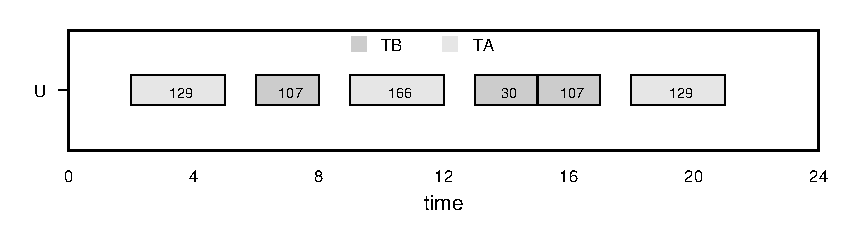
\includegraphics{SS_gantt.pdf}
\caption{Periodic production schedule to respond to nominal demands}
\label{fig:gantt_ss}
\end{figure*}

\subsubsection{Dynamic Response}
In this section, we show the dynamic response to a stochastic demand
signal.

We first consider the closed-loop solution, in which, at each sampling
time optimization problem \eqref{eq:PbNT} is solved, and compare it
with the closed-loop solution in which the optimization problem
\eqref{eq:PbT} is solved. In \eqref{eq:PbT}, we force the final state
to lie on the periodic profile $\mathbb{X}_p$. Hence, at the end of
the planning horizon $N$, the supply-chain is at a state from which it
can respond to the nominal demand. In contrast, for the optimization
problem \eqref{eq:PbNT}, the terminal state is chosen without
considering future demands that arrive after the planning horizon
$N$. Therfore, the solutions to \eqref{eq:PbNT} have (i) fewer
production and (ii) lesser inventory at nodes. This leads to
increasing backorders when new demands are observed at the next
sampling time. In Figure \ref{fig:BO_TNT}, we compare the backorders
observed in the closed-loop when the MPC optimizer solved
\eqref{eq:PbNT} and \eqref{eq:PbT}. In Figure \ref{fig:gantt_TNT}, we
show the Gantt chart for the implemented schedule by the two MPCs. The
planning horizon used was $N = 12$. Note that, under the presence of
persistent distrubance (that is different from the nominal
disturbance), the MPC design has to be robust
\citep[Ch 3.]{rawlings:mayne:2009}. In this example, we have not
designed robust-MPC but instead the results show the inherent-robustness of
nonminal MPC to reject small deviations from the nominal
demand. 
 
\begin{alignat}{1}
\label{eq:PbNT}
\mathbb{P}_N(x):& \min_{\bu,x(0)}{\sum_{i=0}^{N-1}\ell_E(x(i),u(i),d_s(i))} \nonumber \\
&\text{s.t~} x(i+1) = Ax(i) + Bu(i)+B_dd_s(i), \nonumber\\
&\underbar{x} \leq x(i) \leq \bar{x},  \\
&\underbar{u} \leq u(i) \leq \bar{u}, \nonumber \\
& \text{Assignment constraint}\eqref{eq:assign} \nonumber\\
& x(0) = x \nonumber\\
&i = 0,1,\ldots,N_p-1\nonumber
\end{alignat}

\begin{alignat}{1}
\label{eq:PbT}
\mathbb{P}_N(x):& \min_{\bu,x(0)}{\sum_{i=0}^{N-1}\ell_E(x(i),u(i),d_s(i))} \nonumber \\
&\text{s.t~} x(i+1) = Ax(i) + Bu(i)+B_dd_s(i), \nonumber\\
&\underbar{x} \leq x(i) \leq \bar{x},  \\
&\underbar{u} \leq u(i) \leq \bar{u}, \nonumber \\
& \text{Assignment constraint}\eqref{eq:assign} \nonumber\\
& x(0) = x \nonumber \\
& x(N) \in \mathbb{X}_p \nonumber\\
&i = 0,1,\ldots,N_p-1\nonumber
\end{alignat}


\begin{figure*}
\begin{center}
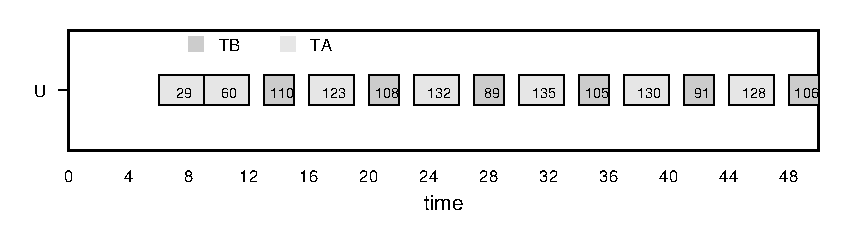
\includegraphics{NTS_gantt.pdf}
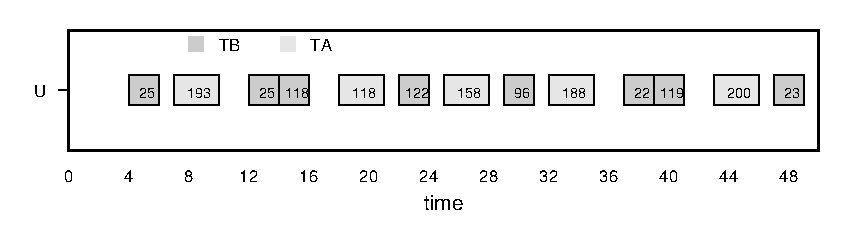
\includegraphics{TS_gantt.pdf}
\caption{Production schedule for the MPC without terminal constraints that optimized
  \eqref{eq:PbNT} (Top) compared with production schedule for the MPC
  with terminal constraints that optimized \eqref{eq:PbT}. Note how larger batches are made for
  the problem with terminal constraints}
\end{center}
\label{fig:gantt_TNT}
\end{figure*}

\begin{figure*}
\centering
\scriptsize
\resizebox{1\textwidth}{!}{% GNUPLOT: LaTeX picture with Postscript
\begingroup
  \makeatletter
  \providecommand\color[2][]{%
    \GenericError{(gnuplot) \space\space\space\@spaces}{%
      Package color not loaded in conjunction with
      terminal option `colourtext'%
    }{See the gnuplot documentation for explanation.%
    }{Either use 'blacktext' in gnuplot or load the package
      color.sty in LaTeX.}%
    \renewcommand\color[2][]{}%
  }%
  \providecommand\includegraphics[2][]{%
    \GenericError{(gnuplot) \space\space\space\@spaces}{%
      Package graphicx or graphics not loaded%
    }{See the gnuplot documentation for explanation.%
    }{The gnuplot epslatex terminal needs graphicx.sty or graphics.sty.}%
    \renewcommand\includegraphics[2][]{}%
  }%
  \providecommand\rotatebox[2]{#2}%
  \@ifundefined{ifGPcolor}{%
    \newif\ifGPcolor
    \GPcolortrue
  }{}%
  \@ifundefined{ifGPblacktext}{%
    \newif\ifGPblacktext
    \GPblacktexttrue
  }{}%
  % define a \g@addto@macro without @ in the name:
  \let\gplgaddtomacro\g@addto@macro
  % define empty templates for all commands taking text:
  \gdef\gplbacktext{}%
  \gdef\gplfronttext{}%
  \makeatother
  \ifGPblacktext
    % no textcolor at all
    \def\colorrgb#1{}%
    \def\colorgray#1{}%
  \else
    % gray or color?
    \ifGPcolor
      \def\colorrgb#1{\color[rgb]{#1}}%
      \def\colorgray#1{\color[gray]{#1}}%
      \expandafter\def\csname LTw\endcsname{\color{white}}%
      \expandafter\def\csname LTb\endcsname{\color{black}}%
      \expandafter\def\csname LTa\endcsname{\color{black}}%
      \expandafter\def\csname LT0\endcsname{\color[rgb]{1,0,0}}%
      \expandafter\def\csname LT1\endcsname{\color[rgb]{0,1,0}}%
      \expandafter\def\csname LT2\endcsname{\color[rgb]{0,0,1}}%
      \expandafter\def\csname LT3\endcsname{\color[rgb]{1,0,1}}%
      \expandafter\def\csname LT4\endcsname{\color[rgb]{0,1,1}}%
      \expandafter\def\csname LT5\endcsname{\color[rgb]{1,1,0}}%
      \expandafter\def\csname LT6\endcsname{\color[rgb]{0,0,0}}%
      \expandafter\def\csname LT7\endcsname{\color[rgb]{1,0.3,0}}%
      \expandafter\def\csname LT8\endcsname{\color[rgb]{0.5,0.5,0.5}}%
    \else
      % gray
      \def\colorrgb#1{\color{black}}%
      \def\colorgray#1{\color[gray]{#1}}%
      \expandafter\def\csname LTw\endcsname{\color{white}}%
      \expandafter\def\csname LTb\endcsname{\color{black}}%
      \expandafter\def\csname LTa\endcsname{\color{black}}%
      \expandafter\def\csname LT0\endcsname{\color{black}}%
      \expandafter\def\csname LT1\endcsname{\color{black}}%
      \expandafter\def\csname LT2\endcsname{\color{black}}%
      \expandafter\def\csname LT3\endcsname{\color{black}}%
      \expandafter\def\csname LT4\endcsname{\color{black}}%
      \expandafter\def\csname LT5\endcsname{\color{black}}%
      \expandafter\def\csname LT6\endcsname{\color{black}}%
      \expandafter\def\csname LT7\endcsname{\color{black}}%
      \expandafter\def\csname LT8\endcsname{\color{black}}%
    \fi
  \fi
  \setlength{\unitlength}{0.0500bp}%
  \begin{picture}(7200.00,3024.00)%
    \gplgaddtomacro\gplbacktext{%
      \csname LTb\endcsname%
      \put(946,714){\makebox(0,0)[r]{\strut{} 0}}%
      \put(946,919){\makebox(0,0)[r]{\strut{} 10}}%
      \put(946,1123){\makebox(0,0)[r]{\strut{} 20}}%
      \put(946,1328){\makebox(0,0)[r]{\strut{} 30}}%
      \put(946,1532){\makebox(0,0)[r]{\strut{} 40}}%
      \put(946,1737){\makebox(0,0)[r]{\strut{} 50}}%
      \put(946,1941){\makebox(0,0)[r]{\strut{} 60}}%
      \put(946,2146){\makebox(0,0)[r]{\strut{} 70}}%
      \put(946,2350){\makebox(0,0)[r]{\strut{} 80}}%
      \put(946,2555){\makebox(0,0)[r]{\strut{} 90}}%
      \put(946,2759){\makebox(0,0)[r]{\strut{} 100}}%
      \put(1078,484){\makebox(0,0){\strut{} 0}}%
      \put(2223,484){\makebox(0,0){\strut{} 10}}%
      \put(3368,484){\makebox(0,0){\strut{} 20}}%
      \put(4513,484){\makebox(0,0){\strut{} 30}}%
      \put(5658,484){\makebox(0,0){\strut{} 40}}%
      \put(6803,484){\makebox(0,0){\strut{} 50}}%
      \put(176,1731){\rotatebox{-270}{\makebox(0,0){\strut{}Backorder -Retailer}}}%
      \put(3940,154){\makebox(0,0){\strut{}Time}}%
    }%
    \gplgaddtomacro\gplfronttext{%
      \csname LTb\endcsname%
      \put(5816,2586){\makebox(0,0)[r]{\strut{}Without terminal constraint}}%
      \csname LTb\endcsname%
      \put(5816,2366){\makebox(0,0)[r]{\strut{}With terminal constraint}}%
    }%
    \gplbacktext
    \put(0,0){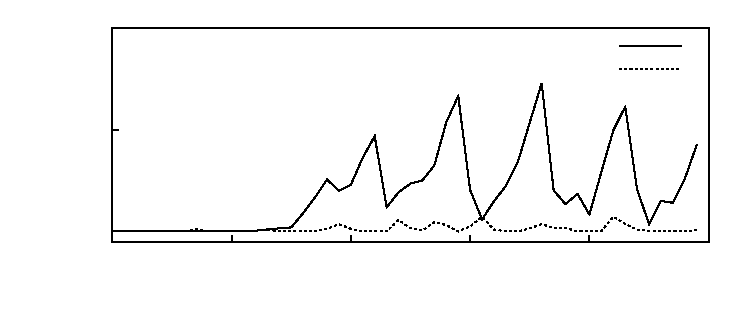
\includegraphics{BOprofile}}%
    \gplfronttext
  \end{picture}%
\endgroup
}
\caption{Combined backorder at all the retailer nodes}
\label{fig:BO_TNT}
\end{figure*}





\section{Conclusions}
\label{sec:conclusions}
In rolling horizon optimization procedure, a cost function is
minimized subject to the dynamics of the system over a finite planning
or prediction horizon. However, if the terminal state of the system at
the end of the prediction horizon is not considered properly; optimal
open-loop solutions can lead to undesirable closed-loop properties. A
vast body of literature has been devoted to designing stable
closed-loop solutions when employing rolling horizon optimization by
identifying terminal state constraints and penalties that often help
us identify a (suboptimal) infinite horizon open-loop solution. These
results include stability theorems for non-linear systems
that minimize a positive definite objective function, and more
recently. stability theorems for  non-linear systems that minimize any
general objective function. 

The main contribution of this paper is to compliment the research in
MPC/ Rolling horizon optimization frameworks for supply chain
management by (i) showing the desirable properties of algorithms that
guarantee closed-loop stability and (ii) demonstrating the design of
such control policies for supply chains.  The main message of the paper  is
that future researchers should appreciate the importance of considering the dynamics of the supply
chain, not only in the prediction horizon; but also on the infinite
horizon.

Future work in this field include developing
theory and implementing algorithms for the combined scheduling and
planning problem. We have shown that the standard
scheduling model can be written in the state-space form and identified
terminal conditions that guarantee recursive feasibility. The extension to that
theory would be to utilize results from hybrid dynamic systems to show
Lyapunov stability of a closed-loop scheduling dynamics. 

The stability results in this paper are for nominal demand
scenarios. Practical supply chain operations are always going to
observer stochastic demands. A future extension of the work presented
here would be to develop robust closed-loop solutions in the presence
of uncertain demand. Future work in integrating scheduling models and control
theory also include (i) Finding a general terminal constraint, as
periodic constraints may not even exist for certain scheduling
problems and (ii) Developing supporting MPC theory  including finding
a Lyapunov function to prove convergence and stability.

\bibliographystyle{abbrvnat}
{\bibliography{abbreviations,articles,proceedings,books,unpub}}
\end{document}

